%&pdflatex
\documentclass[12pt]{article}
\usepackage{algorithmicx}
\usepackage[ruled]{algorithm}
\usepackage{algpseudocode}
\usepackage{algpascal}
\usepackage{algc}
\usepackage{url,enumerate, amssymb, anysize, booktabs, amsfonts}
\usepackage[colorlinks = true,
linkcolor = blue,
urlcolor  = blue,
citecolor = green,
anchorcolor = blue]{hyperref}
\usepackage{setspace,listings}
\usepackage[dvipdfmx]{graphicx}
\usepackage{amsmath}
\usepackage{psfrag}
\usepackage[font=small,labelfont=bf]{caption}
\usepackage{enumerate}
\usepackage{natbib, subcaption}
\usepackage{url} % not crucial - just used below for the URL 
\usepackage{sidecap}
\sidecaptionvpos{figure}{c}

% NOTE: To produce blinded version, replace "0" with "1" below.
\newcommand{\blind}{0}

%%%%%%%%%% EXACT 1in MARGINS %%%%%%%                                   %%
\setlength{\textwidth}{6.5in}     %%                                   %%
\setlength{\oddsidemargin}{0in}   %% (It is recommended that you       %%
\setlength{\evensidemargin}{0in}  %%  not change these parameters,     %%
\setlength{\textheight}{8.5in}    %%  at the risk of having your       %%
\setlength{\topmargin}{0in}       %%  proposal dismissed on the basis  %%
\setlength{\headheight}{0in}      %%  of incorrect formatting!!!)      %%
\setlength{\headsep}{0in}         %%                                   %%
\setlength{\footskip}{.5in}       %%                                   %%
%%%%%%%%%%%%%%%%%%%%%%%%%%%%%%%%%%%% 
\usepackage{color,amssymb}
\usepackage{fancyhdr, mathtools}
\usepackage{dcolumn}
\usepackage{indentfirst, verbatim}
%\newcounter{equationset, sectsty, breqn}
\usepackage{setspace,float,lscape,amsmath,color}
\usepackage{color,amssymb}
\usepackage{fancyhdr, mathtools, amsthm}
\theoremstyle{definition}
\newtheorem{definition}{Definition}[section]
\newtheorem{theorem}{Theorem}[section]
\newtheorem{corollary}{Corollary}[theorem]
\newtheorem{lemma}[theorem]{Lemma}
\newtheorem{remark}{Remark}


\newcommand{\Linefor}[2]{%
	\State \algorithmicfor\ {#1}\ \algorithmicdo\ {#2} \algorithmicend\ \algorithmicfor%
}
\newcommand{\Lineif}[2]{%
	\State \algorithmicif\ {#1}\ \algorithmicdo\ {#2} \algorithmicend\ \algorithmicif%
}


\renewcommand{\algorithmicrequire}{\textbf{Input:}}
\renewcommand{\algorithmicensure}{\textbf{Output:}}

%\usepackage{algorithmicx}

%\algdisablelines

\begin{document}
	
	%\bibliographystyle{natbib}
	
	\def\spacingset#1{\renewcommand{\baselinestretch}%
		{#1}\small\normalsize} \spacingset{1}
	
	
	%%%%%%%%%%%%%%%%%%%%%%%%%%%%%%%%%%%%%%%%%%%%%%%%%%%%%%%%%%%%%%%%%%%%%%%%%%%%%%
	
	\if1\blind
	{
		\title{\bf Testing independence in networks via family of network metrics}
		\author{Youjin Lee\thanks{
				The authors gratefully acknowledge \textit{please remember to list all relevant funding sources in the unblinded version}}\hspace{.2cm}\\
			Department of Biostatistics, Johns Hopkins School of Public Health\\
			and \\
			Author 2 \\
			Department of ZZZ, University of WWW}
		\maketitle
	} \fi
	
	\if0\blind
	{
		\bigskip
		\bigskip
		\bigskip
		\begin{center}
			{\LARGE\bf Testing independence in networks via family of network metrics}
		\end{center}
		\medskip
	} \fi
	
	
\sloppy
\bigskip
\begin{abstract}
	%The text of your abstract. 200 or fewer words.
Propelled by increasing demand and supply in network data, investigating whether network structures are associated with the attributes of interest has been an important concern in natural or social science. We consider the problem of network dependence, which refers to any types of dependence between network topology and its nodal attributes and propose the method to test network independence. However due to the interdependency in constructing network, standard independence test cannot be directly applied but instead the former network independence tests have introduced network models primarily focusing on globally persistent dependence. To overcome these challenges, we introduce a nonparametric multiscale test statistic which is robust to both high dimensionality and nonlinearity by utilizing a family of network geometries. Our simulation studies demonstrate the outstanding performance of the method under various circumstances. We also suggest the measure to quantify each node's contribution to detecting dependency, which is applied to the political network in the end.
\end{abstract}
	
	\noindent%
	{\it Keywords:} distance correlation, multiscale generalized correlation, diffusion maps, exchangeable graph, stochastic block model 
	\vfill
	
	\newpage
	\spacingset{1.45} % DON'T change the spacing!
	\section{Introduction}
	\label{sec:intro}

%% dependence over network
Statisticians have long considered the problem of revealing the relationship between two different data sets. Above all determining the existence of any association or any dependence would be the first step in characterizing the relationship. Independence test between two univariate random variables, for example, could start from deriving a correlation coefficient or estimating a coefficient from linear regression model. However as types of data have diversified or dimension of the data has increased, various forms of multivariate independence tests have been suggested~\citep{heller2012consistent, szekely2007measuring}. We consider independence test upon \textbf{non-traditional but ubiquitous dataset of \textit{network} which is very likely to possess the properties of both high dimensionality and nonlinearity}. Network, formally defined as a collection of nodes and edges, has been suffered from a dearth of proper analysis due to its distinct way to be constructed. In this paper we define any kinds of dependency between network topology and nodal attributes as \textit{network dependence} and propose a method to test network independence considering unique properties of network. 

% literature reviews about testing network independence. 
\textbf{The literature on detecting dependency between network and nodal attributes has primarily focused on their relationship explained only by network model under the boundary of model assumption} \citep{wasserman1996logit, howard2016understanding, christakis2007spread, christakis2008collective}. A fundamental difficulty of model-based independence tests comes from the fact that not all networks follow the structures described by known network models. \cite{fosdick2015testing} overcomes this issue by estimating network factors which are believed to embody each node's locations in network space. These factors are in the end used to test independence between network topology and nodal attributes by implementing standard statistical testing method. Through allowing us to choose the dimension of latent factors, they make up the constraints of parametric modeling. However their statistical modeling on networks still rely on the assumption that all the nodes in network would follow the same pattern of dependence -- subject to additive and multiplicative effect. In real network data, on the other hand, \textbf{it is very common that not all nodes exhibit the same pattern of dependence on their network relationship and also the amount of reliance on network may differ among them.}

\begin{figure}[h]
	\centering
	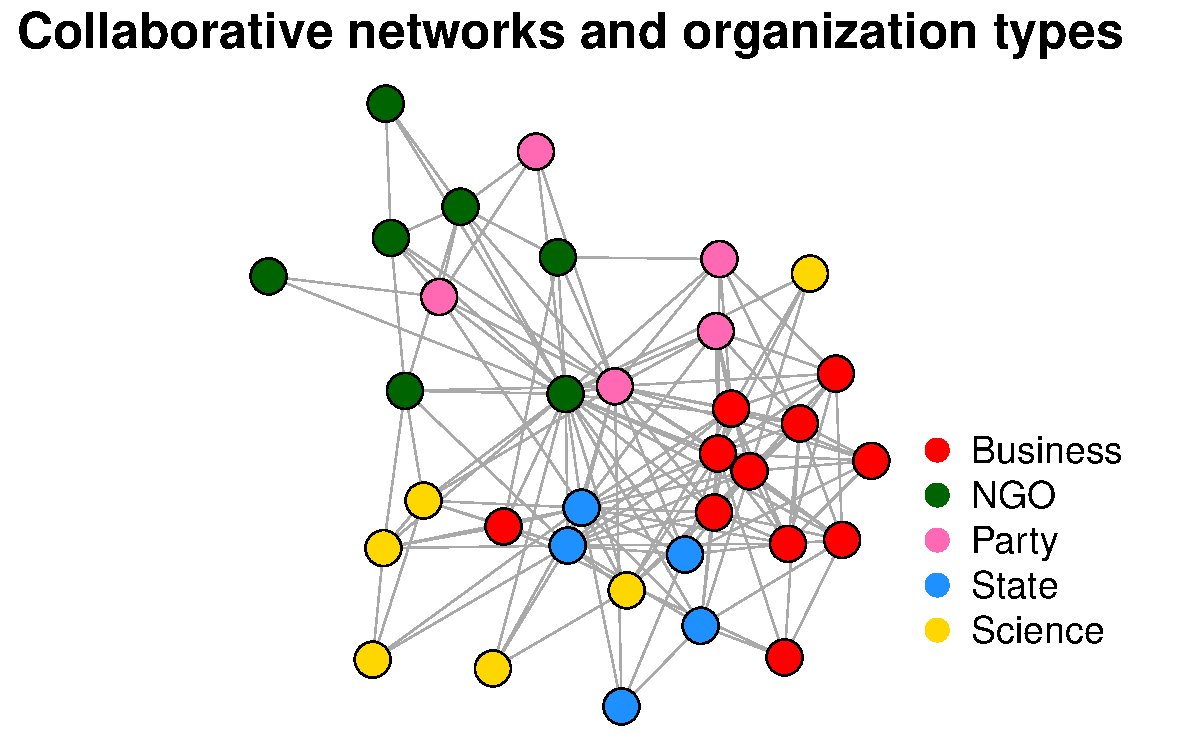
\includegraphics[width=4in]{../../Figure/introplot.pdf}	
	\caption{You may conjecture that organizations with the same type are more likely to collaborate each other at first glance; but there has been a lack of statistical method to test if there exists any significant relationship between network topology and node-specific attributes and if any, which node exerts the most dependency on network.}
	\label{fig:intro}
\end{figure}

% bulleted list of 3-5 main challenges that must be overcome.
\textbf{Different from a random vector, network or equivalently graph involves a particular construction which we should take into account.} Throughout this paper, we assume that we are given an unweighted and undirected, connected network, equivalently a graph $\mathbf{G}$ without self-loop, comprised of $n (\in \mathbb{N})$ nodes. An adjacency matrix of this given network, denoted by $A = \{A_{ij} : i,j= 1,..,n \}$, is to formalize the relational data of network, where $A_{ij} = 1$ if node $i$ and node $j$ are adjacent each other and zero otherwise. Let us define a $m$-variate ($m \in \mathbb{N}$) random variable associated with each node, i.e. nodal attributes, $\mathbf{X}  \in \mathbb{R}^{m}$ which we are interested in. Investigating correlation between $\mathbf{G}$ and $\mathbf{X}$, i.e. testing whether their distributions are independent or not is a key focus in our study. An observed network $\mathbf{G}$ can represent social network of students within a school and $\mathbf{X}$ is student-specific grades or heights, for example; or $\mathbf{G}$ can be a collaboration network and $\mathbf{X}$ denotes some properties of participants under collaboration as in Figure~\ref{fig:intro}.  We aim to detecting significant association between network topology configured in $\mathbf{G}$ and nodal attributes $\mathbf{X}$ whatever the true nature of network is and however the network is correlated with $\mathbf{X}$. We first have to consider increasing amount of information inherent in network data as the number of nodes increases, which might lead to diverse pattern in dependency as well. In addition, by its definition, an adjacency matrix $A$ involves dependency among its columns and row, so thus we may not utilize an adjacency matrix directly when required independent observations.
	
% 2-3 summary of what you did.	
\textbf{To overcome these challenges, we propose applying distance-based statistic called multiscale generalized correlation (\texttt{MGC})~\citep{shen2016discovering} into testing network independnece which deals with correlation between high dimensional data sets possibly having nonlinear dependence.} However we still confront with the difficulty in finding the valid \textit{i.i.d} node-specific coordinates of which Euclidean distance will be an ingredient for the statistics. We claim that graph geometries derived from random walk on graph furnish robust network metrics against to increased variability in edge distributions as well as they satisfy theoretical constraints.
	
% 2-3 sentence summary on how your work changes the world. 
\textbf{In this paper, beyond the traditional setting of the data in independence test, e.g. between two random vectors, we suggest the method to investigate unique but also ubiquitous data of network and its nodal attributes by utilizing the method testing two random vectors.} By suggesting using a family of network metrics which are equipped with favored theoretical and practical properties, we are able to better understand relative locations of each node over network. We are going to elaborate the statistic and demonstrate its validity under some network metrics in Section~\ref{sec:method}. In Section~\ref{sec:sim}, simulation results demonstrate the best performance of our method compared to the existing under various circumstances. Real data example in section~\ref{sec:real} show one of the applications among many.  
	
%%%%%%%%%%%%%%%%%%%%%%%%%%%%%%%%%%%%%%%%%%
\bigskip
\section{Methodology}
\label{sec:method}

\subsection{Multiscale Generalized Correlation}

Relationship between network and nodal attributes often exhibits local or nonlinear properties having high dimensionality. For example, it is likely that attributes of some subjects may be affected by their network relationship but those of the others are not; or that attributes are correlated on network only when network relationships are too strong. \cite{szekely2007measuring} extended pairwise constructed generalized correlation coefficient and developed distance correlation (\texttt{dCorr}) statistics which guarantee consistency against all types of dependence even under high dimensional data sets. The test setting starts from given $n \in \mathbb{N}$ pairs of \textit{i.i.d} random samples $\big(  \mathbf{W}, \mathbf{Y}  \big)  = \{ (\mathbf{w}_{i}, \mathbf{y}_{i}) : \mathbf{w}_{i} \in \mathbb{R}^{q}, \mathbf{y}_{i} \in \mathbb{R}^{m}, i = 1,...,n \}$. Define $C_{ij} = \parallel \mathbf{w}_{i} - \mathbf{w}_{j} \parallel$ and $D_{ij} = \parallel \mathbf{y}_{i} - \mathbf{y}_{j} \parallel$ for $i,j=1,2, \ldots ,n$, where $\parallel \cdot \parallel$ is an Euclidean distance. Distance correlation (\texttt{dCorr}) is defined via distance covariance (\texttt{dCov}) $\mathcal{V}^2_{n}$ of $\mathbf{W}$ and $\mathbf{Y}$, which is the following: 
\begin{equation}	 
\mathcal{V}^2_{n}(\mathbf{W}, \mathbf{Y}) = \frac{1}{n^2} \sum\limits_{i,j=1}^{n} \tilde{C}_{ij} \tilde{D}_{ij}.
\end{equation}
Here $\tilde{C}$ and $\tilde{D}$ is doubly-centered $C$ and $D$ by its column mean and row mean respectively. Distance correlation $\mathcal{R}^{2}_{n}(\mathbf{W}, \mathbf{Y})$ is a standardized \texttt{dCov} scaled by $\mathcal{V}^2_{n}(\mathbf{W}, \mathbf{W})$ and $\mathcal{V}^2_{n}(\mathbf{Y}, \mathbf{Y}).$ In addition, a modified distance covariance (\texttt{mCov}) $\mathcal{V}^*_{n}$ and a modified distance correlation (\texttt{mCorr}) $\mathcal{R}^{*}_{n}$ especially for testing high dimensional random vectors were also proposed in \cite{szekely2013distance}. Unfortunately, these correlation measures with nice closed form often fail to capture nonlinear associations especially embedded in high-dimensional data set~\citep{shen2016discovering, heller2012consistent}. Out of this concern, \cite{shen2016discovering} proposed Multiscale Generalized Correlation (\texttt{MGC}) via computing all pairs of local correlation coefficients, excluding distant pairs beyond the certain neighborhood. To be specific, the following set of correlation covariances are calculated:
\begin{equation}
\label{eq:MGC}
{\mathcal{V}^{*}}^2_{n} (\mathbf{W}, \mathbf{Y})_{kl} = \frac{1}{n^2} \sum\limits_{i,j=1}^{n} \tilde{C}_{ij} \tilde{D}_{ij} I \big( r(C_{ij}) \leq k \big) I \big( r(D_{ij}) \leq l  \big) \quad k,l=1,2,..., n ,
\end{equation}
where $r(C_{ij})$ ($r(D_{ij})$) denotes a rank of $\mathbf{w}_{i}$ ($\mathbf{y}_{i}$) relative to $\mathbf{w}_{j}$ ($\mathbf{y}_{j}$), i.e. $r(C_{ij}) = k$ means $w_{i}$ is $w^{'}_{j}$s $k$-nearest friend in terms of Euclidean distance. Based on this set of statistics, MGC finds the best statistic which exhibits the largest correlation between the two data sets. It has already been shown that this local scaled statistic performs no worse than \texttt{dCorr} and that it results improved sensitivity to nonlinear dependence than the distance correlation. We will demonstrate this in Section~\ref{sec:sim}.

\begin{figure}[H]
	\centering
	\begin{subfigure}[b]{0.23\textwidth}
		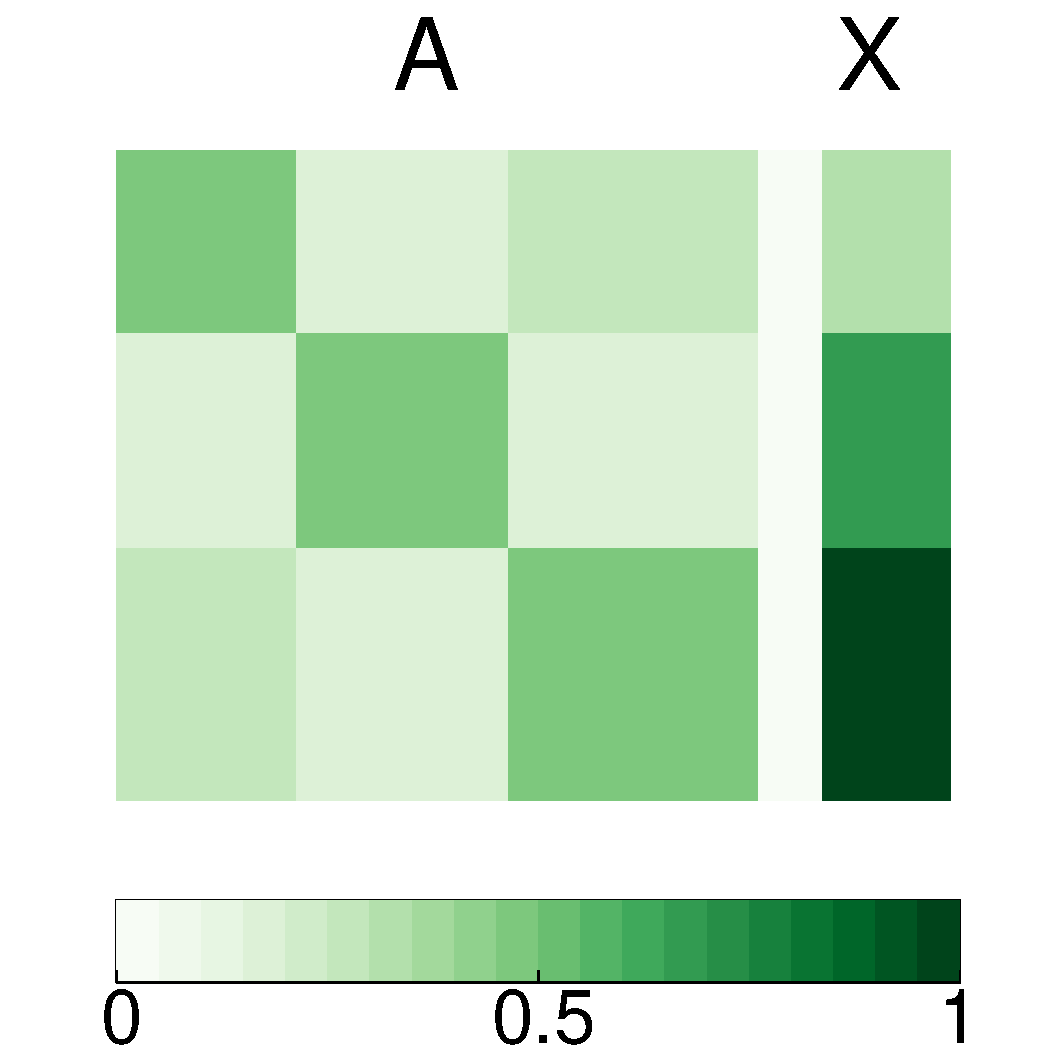
\includegraphics[width=\textwidth]{../../Figure/Pmat.pdf}
		\caption{}
		\label{fig:a}
	\end{subfigure}
	~ %add desired spacing between images, e. g. ~, \quad, \qquad, \hfill etc. 
	%(or a blank line to force the subfigure onto a new line)
	\begin{subfigure}[b]{0.23\textwidth}
		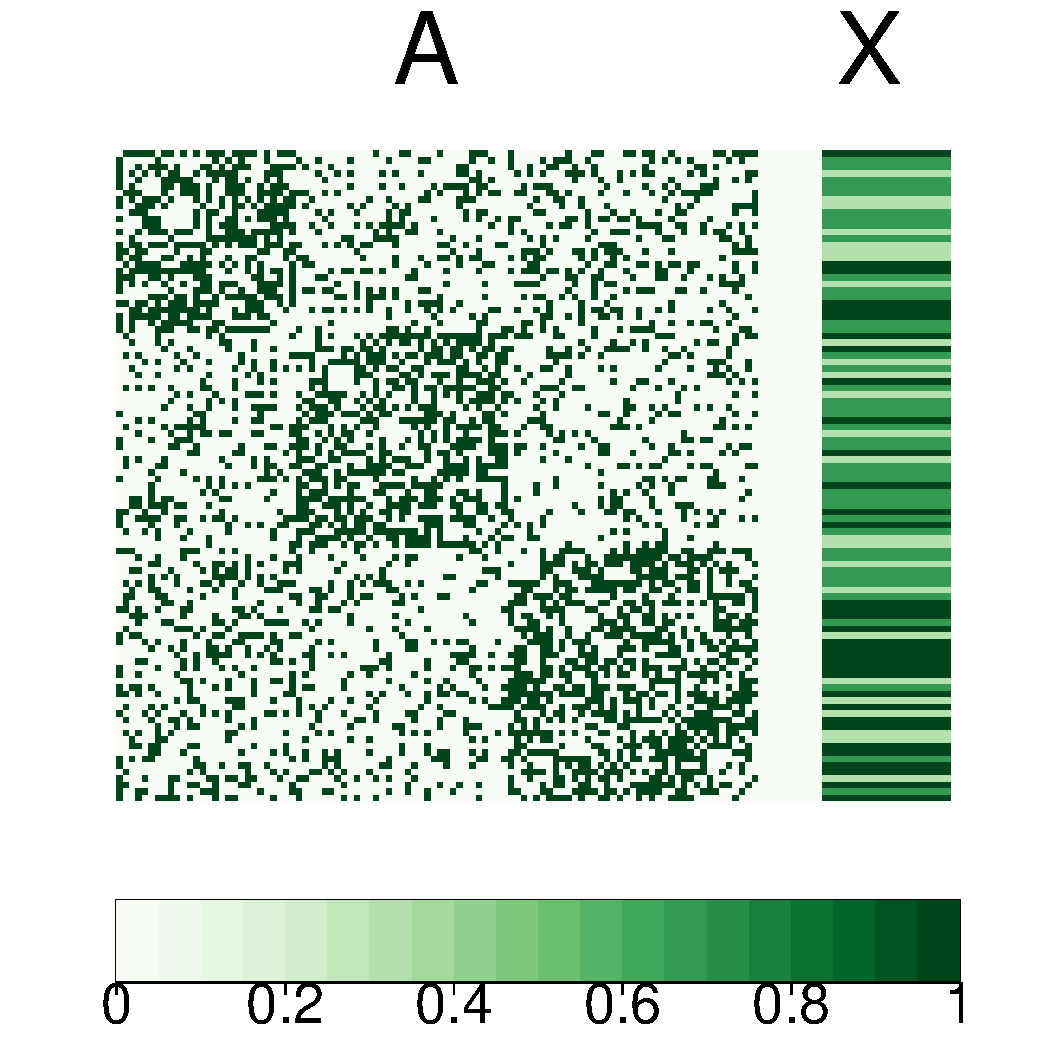
\includegraphics[width=\textwidth]{../../Figure/Amat.pdf}
			\caption{}
		\label{fig:b}
	\end{subfigure}
	~ %add desired spacing between images, e. g. ~, \quad, \qquad, \hfill etc. 
	%(or a blank line to force the subfigure onto a new line)
	\begin{subfigure}[b]{0.23\textwidth}
		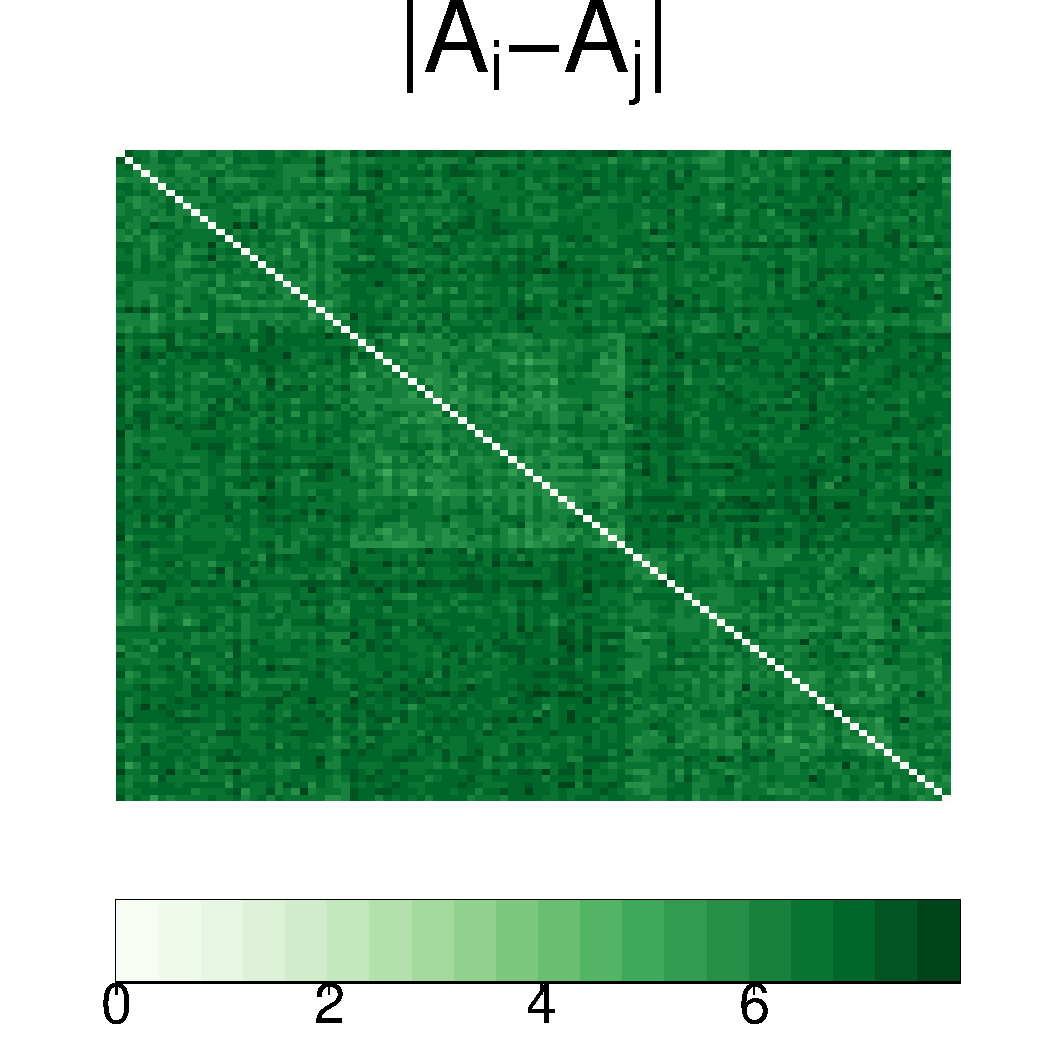
\includegraphics[width=\textwidth]{../../Figure/distA.pdf}
			\caption{}
		\label{fig:c}
	\end{subfigure}
		\begin{subfigure}[b]{0.23\textwidth}
			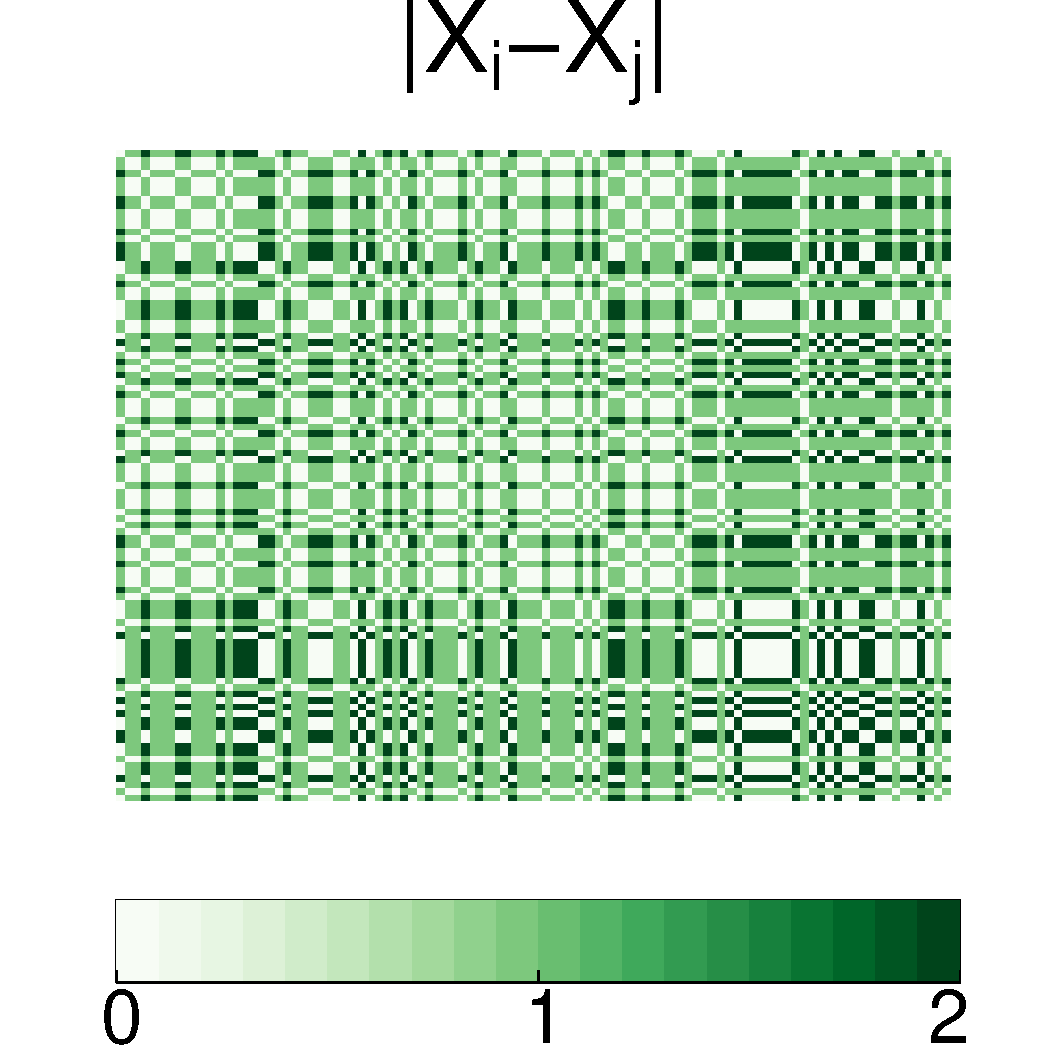
\includegraphics[width=\textwidth]{../../Figure/distX.pdf}
				\caption{}
			\label{fig:d}
		\end{subfigure}
	\caption{Assume that a set of edges follow certain stochastic block model, also depending on the distribution function of nodal attributes $X$ (a), then with some amount of noise we have a realized adjacency matrix and a set of attribute outcomes (b) of which Euclidean distances ((c) $\&$ (d)) are suggested to be used in standard distance-based independence test but neither of them manifests block structures evident in the data generating model.}
	\label{fig:matrics}
\end{figure}

When we are given multivariate, real valued nodal attributes $\mathbf{X}$, its Euclidean distance is easily constructed. However which random vector we should use as a configuration of network $\mathbf{G}$ so what would be the network-base distance are still remaining questions. To be specific, we are required to find \textit{i.i.d} node-specific coordinates of which Euclidean distance reflects a network-based distance between nodes (We are not always required Euclidean metric \citep{lyons2013distance} but discussion on this is out of scope for this paper). You might first propose directly using a column of an adjacency matrix since an adjacency matrix inherits every edge distribution with certain amount of noise. Then we have a $n$-pair of observations $\big\{ \big( \mathbf{A}_{i \cdot} , \mathbf{X}_{i} \big) : \mathbf{A}_{i \cdot} = (A_{i 1} , ... , A_{i n} ) \in \mathbb{R}^{n}, \mathbf{X}_{i} \in \mathbb{R}^{m}, i=1,...,n  \big\}$ as Figure \ref{fig:matrics}. In fact, the main downside of using adjacency matrix is that $\{ \mathbf{A_{i \cdot}}  \}$ cannot enjoy independent samples in an undirected graph. Even if it is in directed graph, there is a lack of reasonable interpretation behind using Euclidean distance of $A$ as a distance matrix in \texttt{MGC} statistics. 
	
\subsection{Exchangeable Graph}

In order to guarantee the requirement of being \textit{i.i.d} edge distribution, we are going to restrict applicable network to a family of graphs which are \textit{exchangeable}. A graph $\mathbf{G}$ is called exchangeable if and only if its adjacency matrix $\mathbf{A}$ is jointly exchangeable \citep{orbanz2015bayesian}. 
	
\begin{definition}[2-array exchangeability]
	\label{exchangeability}
	A random 2-array $(A_{ij})$ is called jointly exchangeable if 
	$$(A_{ij}) \stackrel{d}{=} (A_{\sigma(i) \sigma(j)})$$
	for every permutation $\sigma$ of $n$.
\end{definition}
Even though exchangeability itself cannot guarantee being \textit{i.i.d}, thanks to the celebrated  \textit{de Finetti}~\ref{finetti}'s representation theorem, it has been shown that a sequence of exchangeable variables are \textit{i.i.d} conditioned on its underlying distribution \textit{if and only if} the sequence is exchangeable \citep{orbanz2015bayesian, caron2014sparse}. \textit{Aldous-Hoover theorem}~\ref{Aldous_Hoover} is the representation theorem of 2-array exchangeable array, which is useful to explain jointly exchangeable adjacent matrix. Exchangeable graph is commonly called \textit{graphon} \citep{lovasz2006limits}, which is defined through a random measurable functions \citep{chan2013estimation}.	
\begin{definition}[graphon]
	\label{graphon}
		
	A \textit{graphon} with $n (\in \mathbb{N})$ nodes is defined as a function of a symmetric measurable function $g : [0,1]^2 \rightarrow [0,1]$ with input of $u_{i} \overset{i.i.d}{\sim} Uniform[0,1], i = 1,2,... ,n$. 
	Let $A$ be an adjacency matrix of graphon. Then for any $i < j, \quad i,j=1,2,...,n$:	
\begin{equation}
	Pr \big(   A_{ij} = 1 \big| u_{i}, u_{j} \big) = g \big(  u_{i}, u_{j} \big)
\end{equation}
\end{definition}
By \textit{Aldous-Hoover theorem}, we obtain a clear representation of exchangeable network through measurable function $g$ for a half of the edge set under an undirected network where $A_{ij} = A_{ji}$  $(i,j=1,2,... , n)$. 	
\begin{equation}
( A_{ij} )  =  (   A_{\sigma(i) \sigma(j)}  ) \Longleftrightarrow A_{ij} \overset{i.i.d}{\sim} Bern\big( E_{U} \big[  g(u_{i}, u_{j})   \big] \big),  \quad i < j
\end{equation}  	
Networks based on  widely used graphical model are exchangeable. One of the most popular models is Stochastic Block Model (SBM) \citep{holland1983stochastic} where many of network methodologies have been built on. In the simplest setting of SBM, we assume that each $n$ nodes of $\mathbf{G}$ belongs to one of $K \in \mathbb{N} (\leq n)$ blocks or groups. Block affiliation is important in that the probability of having edges between a pair of nodes depends on which blocks they are in.  Let a latent variable $Z$ indicate each node's block affiliation such that $Z_{1}, Z_{2}, ... , Z_{n} \overset{i.i.d.}{\sim} Multinomial\big( \pi_{1}, \pi_{2}, ... , \pi_{K} \big)$. Then the upper triangular entries of $A$ are independent and identically distributed conditional on $\{\mathbf{Z}\}$:
	\begin{equation} 
	A_{ij} \big| Z_{i}, Z_{j} \overset{i.i.d.}{\sim} Bern\big( \sum\limits_{k,l=1}^{K} p_{kl} I\big( Z_{i} = k, Z_{j} = l  \big)    \big), \forall  i < j.
	\end{equation}
The above distribution can also be represented through some random function $g : [0,1]^2 \rightarrow [0,1]$, e.g.$g\big( W_{i}, W_{j} \big) = \sum\limits_{k,l=1}^{K} p_{kl} I \left( W_{i} \in \big[ \sum\limits_{j=0}^{k-1} \pi_{j}, \sum\limits_{j=0}^{k} \pi_{j}   \big] , W_{j} \in \big[ \sum\limits_{j=0}^{l-1} \pi_{j}, \sum\limits_{j=0}^{l} \pi_{j}  \big]  \right)$ for  $W_{1}, W_{2}, ... , W_{n} \overset{i.i.d.}{\sim} Unif[0,1]$, where $\pi_{0} = 0$ and $\sum\limits_{j=0}^{K}  \pi_{j} = 1$. Then we can have conditional \textit{i.i.d} edge distribution given $g$, restrictive to upper triangular part of $A$.
\begin{equation} 
\begin{gathered}
A_{ij} \big| g, W_{i}, W_{j} \overset{ind}{\sim} Bern \big( g(W_{i}, W_{j})  \big), \forall i < j \\ 
A_{ij} \big| g \overset{i.i.d}{\sim} \int \int Bern \big( g(W_{i}, W_{j}) \big) f_{W}(w_{i}) f_{W}(w_{j}) dw dw, \quad \forall i < j.  
\end{gathered}
\end{equation}
Even though this is not the only representation of edge distribution, for any exchangeable graphs, including SBM and also Random Dot Product Graph (RDPG)~\citep{young2007random}, there must exist a random function $g$ which edges are independent identically distributed conditioning on. 

Despite its advantage on simple representation, graphon is either dense, i.e. $|E| = o(|V|^2)$~\citep{veitch2015class}, or empty. This implies a graphon often fails to represent real network data where sparsity or scale-free distribution is fairly common. Thus, in addition to graphon, we introduce a concept of \textit{graphex}, first proposed by \cite{veitch2015class}, which is more generalized version of graphon and also includes sparse exchangeable graphs \citep{caron2014sparse}.  \cite{caron2014sparse} suggested formalizing a network as point process over $\mathbb{R}^2_{+}$ on the basis of \textit{Kallengerg Representation Theorem} \citep{kallenberg1990exchangeable}. As we were able to conditionally represent $\{ A_{ij} \}$ through a random transformation of \textit{i.i.d} uniform variables, jointly exchangeable point processing network also can be formalized via a random function of \textit{i.i.d} unit rate Poisson process and of \textit{i.i.d} uniform variables. 
To be specific, an undirected graph on a point process on $\mathbb{R}^2_{+}$ can be thought of having an adjacency matrix defined on an edge set $\{ \theta_{i} :  \theta_{i}  \overset{i.i.d}{\sim}  Poisson(1), i = 1,2,\ldots \}$~\citep{kallenberg1990exchangeable}:
\begin{equation}
A_{\theta_{i} \theta_{j}} \overset{i.i.d}{\sim} g(\vartheta_{i}, \vartheta_{j}), \quad i < j,
\label{eq:graphon}
\end{equation}
where $g : \mathbb{R}^{2}_{+} \rightarrow [0,1]$ is a random function defined on unit-rate Poisson processing $\{ \vartheta \}$. In a graphex, joint exchangeability applied to a point processed nodal label $\theta$, not on a node label itself. Despite its more intricate form, representation of sparse graph as exchangeable formation helps us to demonstrate the validity of our proposed methods in real network data. 
\begin{definition}[Joint exchangeability on point process]
	\label{point}
	Let $h > 0$ and  $V_{i} = [h(i-1), hi ]$ for $i \in \mathbb{N}$ then
	\begin{equation}
	\big( A( V_{i} \times V_{j}  )   \big)  \stackrel{d}{=} \big( A( V_{\sigma(i)} \times V_{\sigma(j)}     \big)
	\end{equation}	
	for any permutation $\sigma$ of $\mathbb{N}$.		
\end{definition}

%%%%%%%%%%%%%%%%%%%%%%%%%%%%%%%%%%%
\subsection{Family of Network Distances and Test Statistics}	

Then which network-specific distance should be applied for an exchangeable graph? \cite{coifman2006diffusion} proposed multiscale geometries of data called \textit{diffusion maps}, which inherit every local relation between the nodes when applied in network. The geometries in network are constructed via running random walk on graph by iterating transition matrix of Markov process. Roughly speaking, we go on the journey starting from each node and at each iteration we can cross over one edge. At each iterating time, called \textit{diffusion time}, we calculates the chance to stay between node $i$ and node $j$ considering all possible paths between them, which is assumed to be proportional to the distance. For example, at diffusion time $t$, we travel from each node to others at most $t$ geodesic distance apart. Corresponding location or coordinates of each node at every iteration can be derived as a family of \textit{diffusion maps}. Diffusion maps are constructed by eigenvectors of Markov matrix of which Euclidean distance is called a diffusion distance. For each diffusion time $t \in \mathbb{N}$, we can define a diffusion distance $C_{t}$, using a discrete set of real nonzero eigenvalues $\{ \lambda_{r} \}$ and eigenvectors $\{ \phi_{r}  \}$ of a transition matrix~\citep{coifman2006diffusion,lafon2006diffusion}. 
\begin{equation}
\label{eq:diffusion}
C^2_{t}[i,j]  :=   \parallel \mathbf{U}_{t}(i) - \mathbf{U}_{t}(j) \parallel   \quad i,j = 1,2, \ldots , n
\end{equation}
where $\mathbf{U}_{t}(i) = \begin{pmatrix} \lambda^{t}_{1} \phi_{1}(i) & \lambda^{t}_{2} \phi_{2} (i)  & \ldots & \lambda^{t}_{q} \phi_{q}(i) \end{pmatrix}^{T} \in \mathbb{R}^{q}$ is a diffusion map at time $t$. As diffusion time $t$ increases, distance matrix $C_{t}$ is more likely to take into account distance between two nodes which are relatively difficult to reach each other. Figure~\ref{fig:diffusions} shows three exemplary distance matrices among whole one-parameter family of distance $\{ C_{t} : t \in \mathbb{N} \}$. 

There are two main merits in using a set of diffusion distances under exchangeable graphs: First of all, compared to an adjacency relationship or geodesic distance which are two extremes, diffusion distance well reflects the connectivity since it takes into account every possible path between the two nodes. Second, each diffusion map provides \textit{i.i.d} multivariate coordinates of nodes so that using diffusion distance in distance-based test statistics is a valid method. The following Lemmas show how $\mathbf{U}_{t}$ retains (conditional) independence privileged to exchangeable graph. 
\begin{figure}[H]
	\centering
	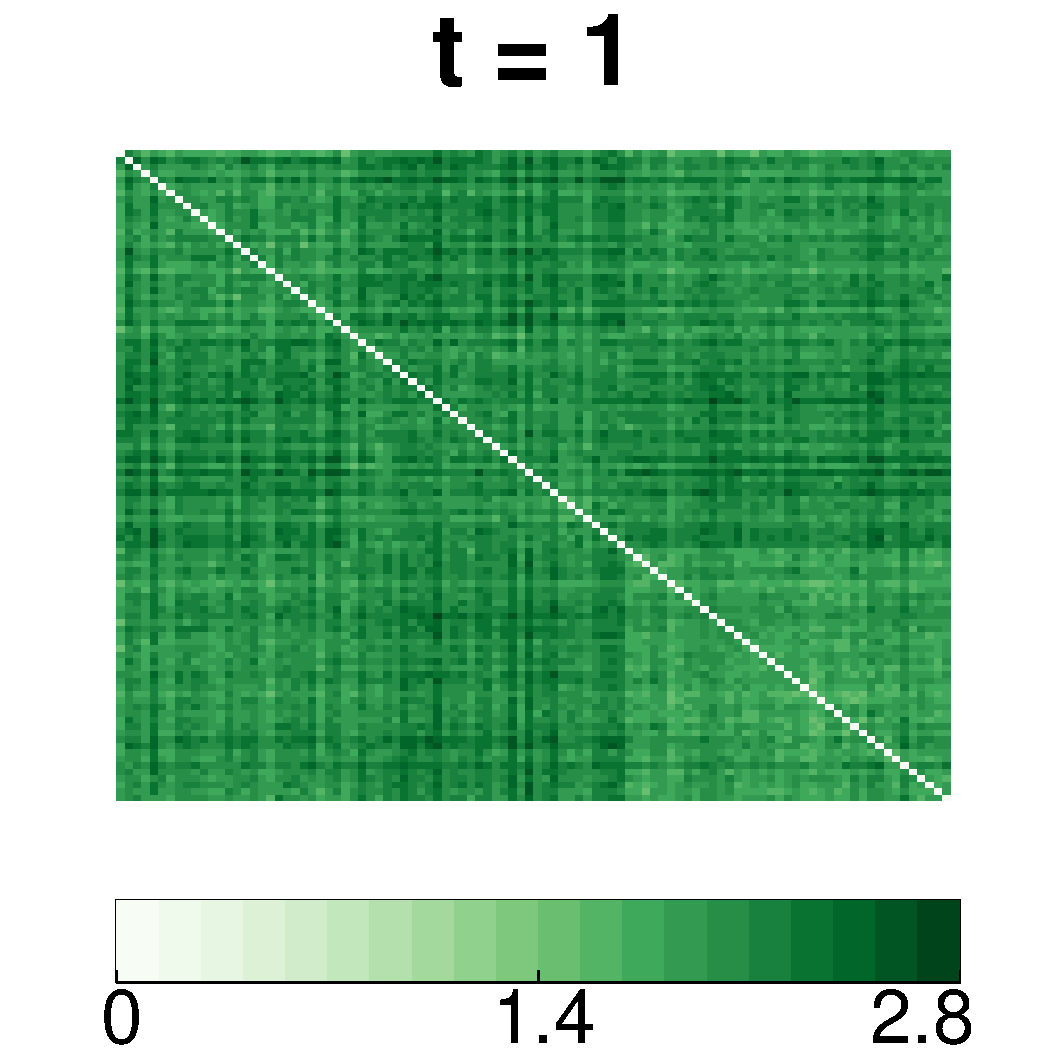
\includegraphics[width=0.3\linewidth]{../../Figure/Dx1.pdf}
	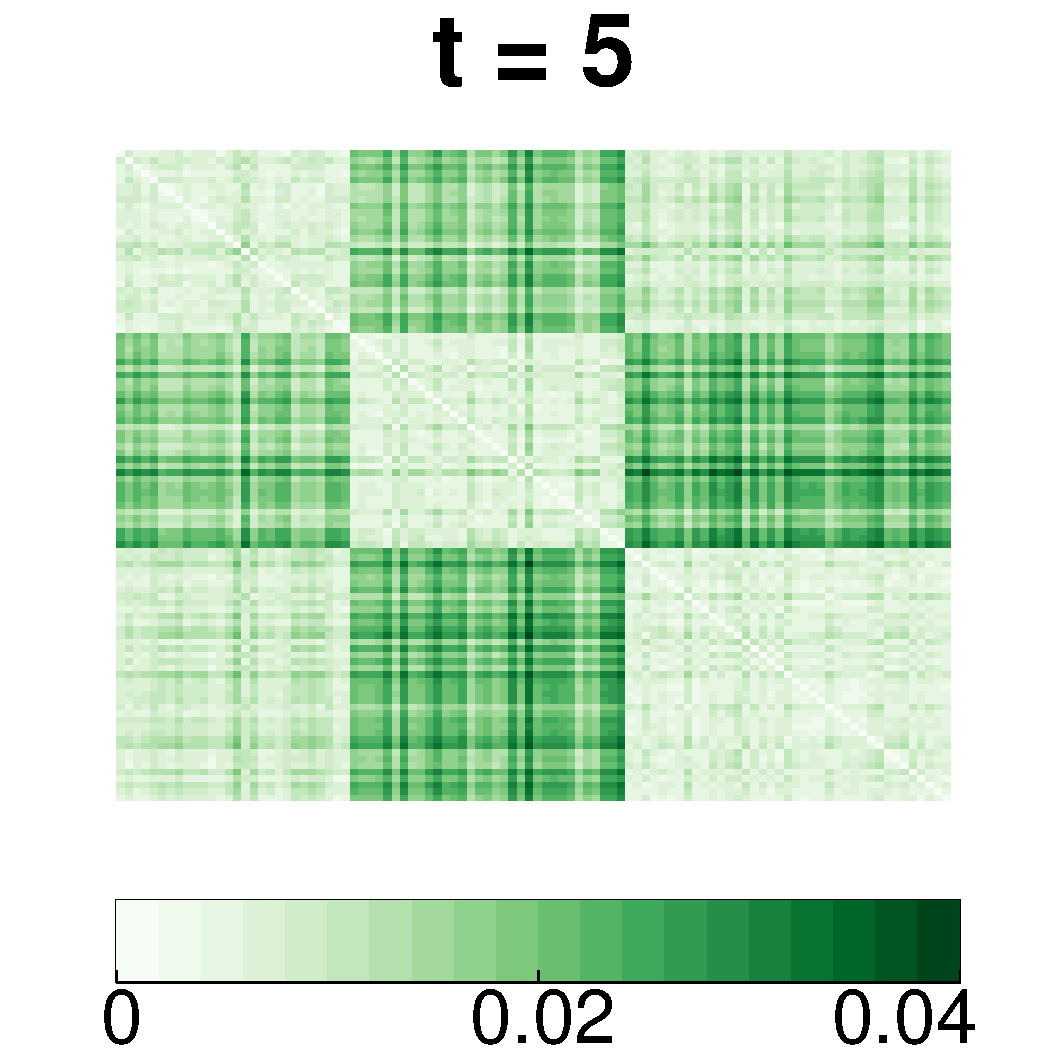
\includegraphics[width=0.3\linewidth]{../../Figure/Dx5.pdf}
	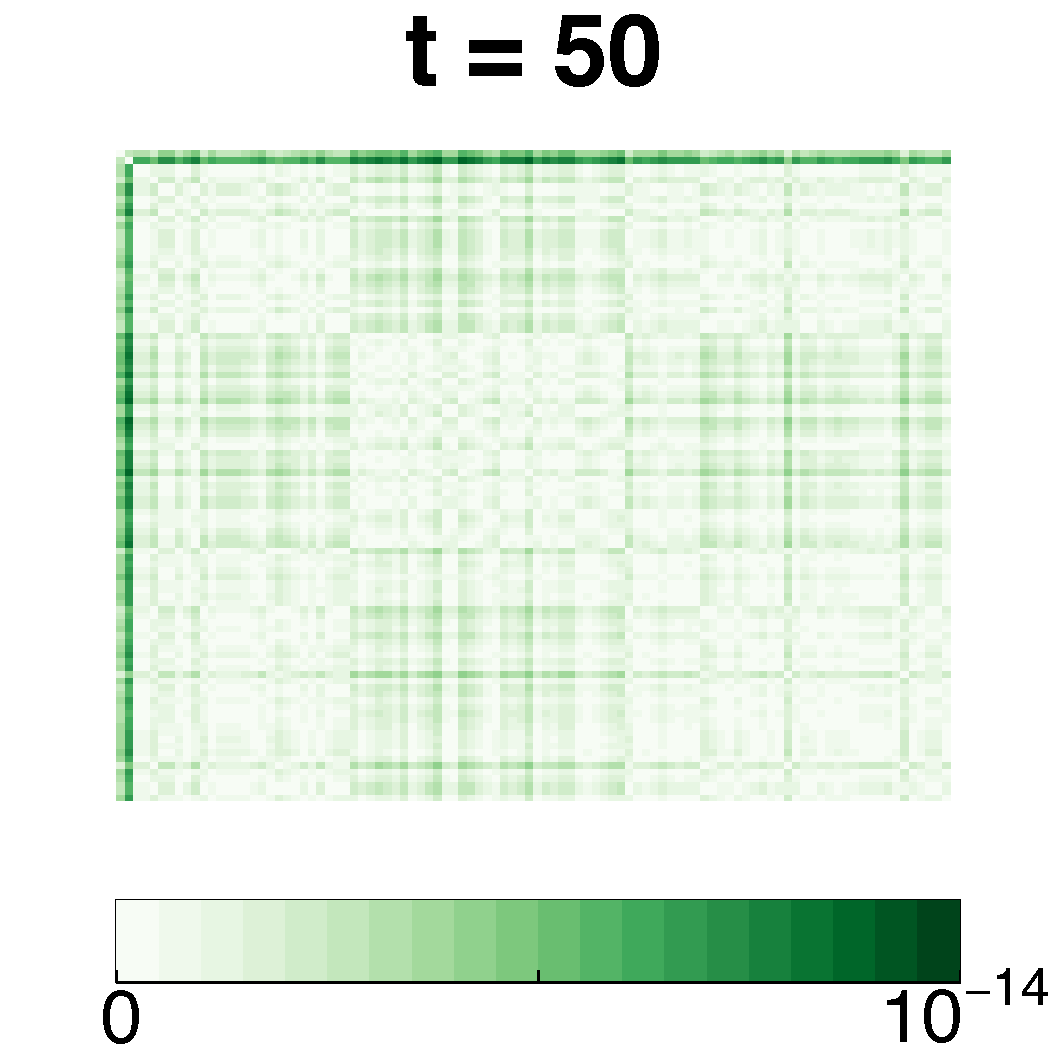
\includegraphics[width=0.3\linewidth]{../../Figure/Dx50.pdf}
	\caption{\textit{Diffusion matrix}, as a proposed alternative for Euclidean distance of $A$, provides \textbf{one-parameter family of network-based distances} where at early stage, e.g. at $t=1$, distance matrix is very similar to Euclidean distance of $A$ but as time goes by the pattern shown in the distance matrix changes, and \textbf{at optimal time point $t^{*} = 5$ distance matrix shows most clear block structures and at the same time it exhibits most dependence to distance matrix of $\mathbf{X}$.}}
	\label{fig:diffusions}
\end{figure}	

\begin{lemma}[Exchangeability and \textit{i.i.d} of $A$ in graphon]
	\label{lemma_graphon}
Assume that a connected, undirected and unweighted graph $\mathbf{G}$ is a graphon. Then 2-array of $\{ A_{ij} : i = 1,2,... ,n , i < j \}$ are  \textit{i.i.d} conditioning on some random link function $g : [0,1]^2 \rightarrow [0,1]$. Thus for fixed row (column) of $A$, $\{ A_{i1}, A_{i2}, ... , A_{in} \} \setminus \{ A_{ii} \} $ , $i \in \{ 1,2,... , n \}$ are conditionally \textit{i.i.d} given a random link function $g$ or equivalently, its underlying distribution.  
\end{lemma}
	
\begin{lemma}[Exchangeability and \textit{i.i.d} of $\mathbf{U}_{t}$]
\label{main_lemma}
	Assume that a connected, undirected and unweighted graph $\mathbf{G}$ is a graphon. Then its transition probability so thus diffusion maps at fixed time $t$ also exchangeable, conditional on a link function of graph. Furthermore, by \textit{de Finetti's Theorem}~\ref{finetti}, such diffusion maps at $t$ are conditionally \textit{i.i.d} given its underlying distribution.    
\end{lemma}
	
Lemma~\ref{main_lemma} above provides us with \textit{i.i.d} one-parameter family of $\{ \mathbf{U}_{t} \}_{t \in \mathbb{N}}$ conditional on its underlying distribution. Unfortunately this is a story only applied to an exchangeable graph, which cannot be sparse. In sparse version of exchangeable graphs, i.e. graphex, one more step of conditioning on point process $\mathbf{\theta}$ is needed.  
	
\begin{lemma}[Exchangeability and \textit{i.i.d} of $A$ in graphex]
\label{lemma_graphex}
Assume that a connected, undirected and unweighted graph $\mathbf{G}$ is a graphex. Then 2-array of $\{ A_{ij} : i = 1,2,... ,n , i < j \}$ are  \textit{i.i.d} conditioning on some random link function $g : [0,1]^2 \rightarrow [0,1]$ and unit-Poisson process $\mathbf{\theta}$. Thus for fixed row (column) of $\mathbf{A}$, $\{ A_{i1}, A_{i2}, ... , A_{in} \} \setminus \{ A_{ii} \} $ , $i \in \{ 1,2,... , n \}$ are conditionally \textit{i.i.d} on its underlying distribution, specifically conditioning on random link function $g$ and $\mathbf{\theta}$.  
\end{lemma}	

Similar to Lemma~\ref{main_lemma}, we are able to show exchangeability of a transition matrix in graphex case, which leads to conditional \textit{i.i.d} of its diffusion maps. If exchangeable diffusion maps are applicable to distance-based test statistics, e.g. \texttt{MGC}, we are then able to dispense with obstacles in testing network independence. Assume that we have a finite sample of infinitely exchangeable sequence $(\mathbf{W}, \mathbf{Y}) = \{ ( \mathbf{w}_{i}, \mathbf{y}_{i} ) : i=1,2, \ldots, n \}$, which is identically distributed as $(\mathbf{w}, \mathbf{y})$ with finite second moment. Then, by the properties of exchangeable sequences, there exists some random measure $\theta$ and its probability measure $P$ such that : 
\begin{equation}
\begin{split}
& w_{i} | \theta  \overset{i.i.d}{\sim} \prod\limits_{i=1}^{n} f_{\mathbf{w}_{i} | \theta}(\mathbf{w}_{i} | \theta)  \\
& \int \prod\limits_{i=1}^{n} f_{ \mathbf{w}_{i} | \theta} ( \mathbf{w}_{i} | \theta ) P(d\theta)  \stackrel{d}{=}   \prod\limits_{i=1}^{n} f_{\mathbf{w}}(\mathbf{w}_{i})  \\
& \mathbf{w}_{i}   \overset{i.i.d}{\sim}  f_{\mathbf{w}}(\mathbf{w})  \quad \mbox{ conditioning on the underlying distribution } f_{\mathbf{w}},
\end{split}
\label{eq:iid}
\end{equation}
where $f$ is a random, marginal distribution integrated over $\theta$; same arguments hold for exchangeable $\{ \mathbf{y}_{i}  \}$. The following two Lemmas serve as the foundation for using exchangeable observations in \texttt{MGC}.

\begin{lemma}
	\label{lemma1}
   Under the above conditions, we have 
	\begin{eqnarray*}
		\mathcal{V}^{2}_{n}(\mathbf{W},\mathbf{Y}) &= \|g_{\mathbf{w},\mathbf{y}}^{n}(t,s)-g_{\mathbf{w}}^{n}(t)g_{\mathbf{y}}^{n}(s)\|^{2},
	\end{eqnarray*}
	where $g_{\cdot}^{n}$ is the empirical characteristic function based upon $\{(\mathbf{w}_{i},\mathbf{y}_{i}), i=1,2,...,n\}$
\end{lemma}

\begin{lemma}
	\label{lemma2}
We have 
	\begin{eqnarray}
		\mathcal{V}_{n}^{2}(\mathbf{W},\mathbf{Y}) &\longrightarrow \mathcal{V}^{2}(\mathbf{w},\mathbf{y}) \quad \quad \mbox{ as } n \rightarrow \infty
	\label{eq:conv1}
	\end{eqnarray}
where $\mathcal{V}^{2} (\mathbf{w},\mathbf{y}) := \| g_{\mathbf{w},\mathbf{y}}(t,s) - g_{\mathbf{w}}(t) g_{\mathbf{y}}(s) \|^2$, and $g_{\cdot}$ is a characteristic function, e.g., $g_{\mathbf{w},\mathbf{y}}(t,s) = E\{\exp\{i \left\langle t,\mathbf{w} \right\rangle  +i \left\langle  s,\mathbf{y}\right\rangle \}\}$.
	It follows that 
	\begin{eqnarray}
		\mathcal{V}_{n}^{2}(\mathbf{W},\mathbf{Y}) &\rightarrow 0 \quad \mbox{ as } n \rightarrow \infty
		\label{eq:conv2}
	\end{eqnarray}
	if and only if $g_{\mathbf{w},\mathbf{y}}(t,s) = g_{\mathbf{w}}(t) g_{\mathbf{y}}(s)$, i.e., $\mathbf{w}$ is independent of $\mathbf{y}$.
\end{lemma}
Lemma~\ref{lemma1} and its following Lemma~\ref{lemma2} facilitate the use of distance correlation while satisfying \textit{Theorem 2} in \cite{szekely2007measuring}.  

\begin{theorem}
	Suppose that we are given $n$ pairs of exchangeable observations $(\mathbf{W}, \mathbf{Y}) = \{  (\mathbf{w}_{i}, \mathbf{y}_{i} ) ; i = 1,2, \ldots, n \}$ having finite second moment. Assume $\mathbf{w}_{i} \overset{i.i.d}{\sim} f_{\mathbf{w}}$ and $\mathbf{y}_{i} \overset{i.i.d}{\sim} f_{\mathbf{y}}$ given underlying distribution for $i = 1,2, \ldots, n$. Then
	\begin{eqnarray}
		\mathcal{V}_{n}^{2}(\mathbf{W},\mathbf{Y}) &\longrightarrow 0 \quad \mbox{ as } n \rightarrow \infty
	\end{eqnarray}	
	\textit{if and only if} $\mathbf{w}$ is independent of $\mathbf{y}$. Moreover, \texttt{dCorr} and \texttt{MGC} are consistent for testing dependence between $\mathbf{w}$ and $\mathbf{y}$, i.e., the testing power converges to $1$ asymptotically for any dependency of finite second moment.
	\label{theoremMain}
\end{theorem}

Note that if $\{ \mathbf{w}_{i} : i = 1,2,\ldots, n \}$ are \textit{i.i.d}, they are exchangeable. Thus estimated latent factors, which are assumed \textit{i.i.d} by \cite{fosdick2015testing} can also be applied to Theorem~\ref{theoremMain}. We already have shown that even under undirected network, diffusion maps remain exchangeable at each diffusion time point $t$. 
\begin{theorem}
	\label{theorem2}
	Then \texttt{MGC} is consistent in testing network independence through testing $H_{0}: f_{\mathbf{U}^{(t)} \cdot \mathbf{X}  }  = f_{\mathbf{U^{(t)}}} \cdot f_{\mathbf{X}}$. In particular, the consistency also holds for the estimated latent positions and adjacency matrix of directed network instead of diffusion maps.
\end{theorem}		
Moreover, we are not going to state otherwise but if you assume to be given a unit-Poisson process $\{ \theta_{i} \}_{i=1}^{n}$, you can lead to the same results for sparse graphex as Theorem~\ref{theoremMain}. 

\subsection{Measure for Node Contribution}

On the other hand, in the presence of nonlinear dependency, some nodes often exert more reliance on their attributes than the others. Like other node-specific measure of importance, e.g. centrality,  the amount of each node's leverage on dependence can be of interest. Here we suggest the measure of node's contribution to detecting dependence by utilizing \texttt{MGC} statistic. Let $(k^{*}, l^{*})$ be the optimal neighborhood choice in distance matrix $(C, D)$ respectively.  Denote the contribution of node $v \in V(G)$ to the testing statistic by  $c(\cdot) : v \rightarrow \mathbb{R}$
\begin{equation}
\label{eq:contribution}
c(v) \propto \sum\limits_{j=1}^{n} \tilde{C}_{j v} \tilde{D}_{j v} I \big(  r (C_{j v}) \leq k^{*}  \big) I \big( r (D_{ j v }) \leq l^{*} \big), 
\end{equation}
which is proportional to $v^{th}$ column-sum of the pre-summed test statistic~\ref{eq:MGC}. Note that the deviation of non-negative \texttt{MGC} statistic from zero implies departure from the independence and also note that we truncate the \texttt{dCov} statistics by column entry's rank. Thus $\tilde{C}_{jv} \tilde{D}_{jv}$ would not be truncated if node $j$ $(\in \{ 1,2, \ldots, n \} \setminus v )$ is important to node $v$ and its larger, positive value would contribute to ${\mathcal{V}^{*}_{n}}^2$ more. The statistic $c(v)$ comes out from these observations. We illustrate how this contribution measure works in the next section~\ref{ssec:node}. 

%%%%%%%%%%%%%%%%%%%%%%%%%%%%%%%%%%%%%%%%%%%%%%%%%%%%%%%%%%%%%%%%
\section{Simulation Study}
\label{sec:sim}
	
In the simulation studies, we make a comparison between empirical testing power across various multivariate independence test statistics: \texttt{MGC}, \texttt{dCorr}(\texttt{mCorr}), Heller-Heller-Gorfine (\texttt{HHG}) \citep{heller2012consistent}, and likelihood ratio test of Fosdick and Hoff (\texttt{FH}). For computing statistical power, we used type I error $\alpha = 0.05$ and obtain p-values of each sample network via permutations. For fair comparison between these testing methods, we also present an additive and multiplicative effect model which \texttt{FH} mostly watch for. All the simulation models are illustrated by joint distribution of adjacent matrix $\mathbf{A}$, nodal attributes $\mathbf{X}$, and latent variable $\mathbf{Z}$, which explains dependence structure between $\mathbf{A}$ and $\mathbf{X}$. 
\begin{equation}
\begin{split}
f(\mathbf{A}, \mathbf{X}, \mathbf{Z}) & = f_{A | Z}(\mathbf{A} | \mathbf{Z}) \cdot f_{Z | X}(\mathbf{Z} | \mathbf{X}) \cdot f_{X}(\mathbf{X}) 
\\ & = f_{A | Z}(\mathbf{A} | \mathbf{Z}) \cdot  f_{X | Z}(\mathbf{X} | \mathbf{Z} ) \cdot f_{Z} (\mathbf{Z}) 
\end{split}
\label{eq:joint_model}
\end{equation}	
According to the joint model~\ref{eq:joint_model}, distribution of edges and nodal attributes are correlated only through a node-specific latent variable $\mathbf{Z}$ no matter whether $\mathbf{X}$ is modeled via $\mathbf{Z}$ or vice versa. For each simulated network, empirical power will be derived by comparing observed statistic to the empirical distribution under the null. 
						
\subsection{Stochastic block model}


\begin{SCfigure}[][h]
	\centering
	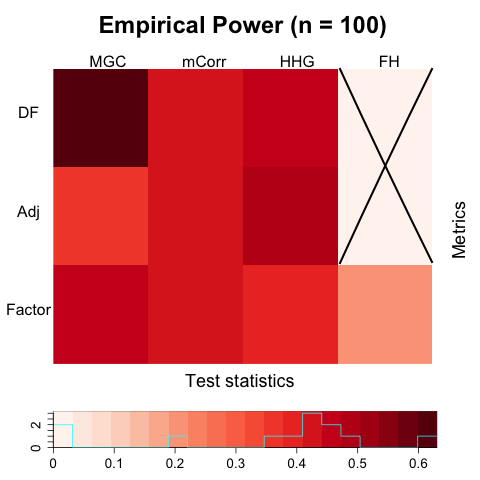
\includegraphics[width=0.4\paperwidth, height=0.4\paperwidth]{../../Figure/ThreeSBM_results_simple.png}
	\caption{This power heatmap illustrates the superior power of multiscale generalized correlation (\texttt{MGC}) under diffusion distance matrix (\texttt{DF}) in three SBM (model~\ref{eq:Three}), compared to under adjacency matrix distance (\texttt{Adj}) or latent factor distance (\texttt{LT}). \textbf{This demonstrates one exemplary network where \texttt{MGC} statistic along with a family of diffusion distances catches non monotonic correlations efficiently than the other statistics and metrics.}}
	\label{fig:threeSBM}
\end{SCfigure}

We already mentioned that Stochastic Block Model (SBM) is one of the most popular and also useful network generative model. We present the SBM with $K=3$ blocks (model~\ref{eq:Three}) where block affiliation for each node is correlated with its attributes $X$. Figure~\ref{fig:threeSBM} illustrates superior performance of \texttt{MGC} as a test statistic combined with diffusion maps (\texttt{DF}) as a network metric. To simply represent model~\ref{eq:Three},
\begin{equation}
E(A_{ij} | X_{i}, X_{j}) = 0.5 I(|X_{i} - X_{j}| = 0) + 0.2 I(|X_{i} - X_{j}| = 1) + 0.3 I(|X_{i} - X_{j}| = 2).
\end{equation}
When $X_{i} = X_{j}$, these two nodes are most likely to have an edge but when $X_{i}$ and  $X_{j}$ differ by one, they are even less likely to have an edge, with probability of 0.2, than the most different pairs of nodes. This actually describes \textbf{nonlinear dependence where \texttt{MGC} is believed to work better than the distance correlation}. To deep into studying performance of local optimal scaled \texttt{MGC} in the presence of both linear dependency and non-linear dependency, we control these two phases through changing a value of $\theta \in (0, 1)$. When $\theta > 0.2$, linear dependency of edge distribution upon nodal attribute $X$ is lost.
\begin{equation}
E(A_{ij} | X_{i}, X_{j}) = 0.5 I(|X_{i} - X_{j}| = 0) + 0.2 I(|X_{i} - X_{j}| = 1) + \theta I(|X_{i} - X_{j}| = 2)
\end{equation}
\begin{figure}[h]
	\centering
	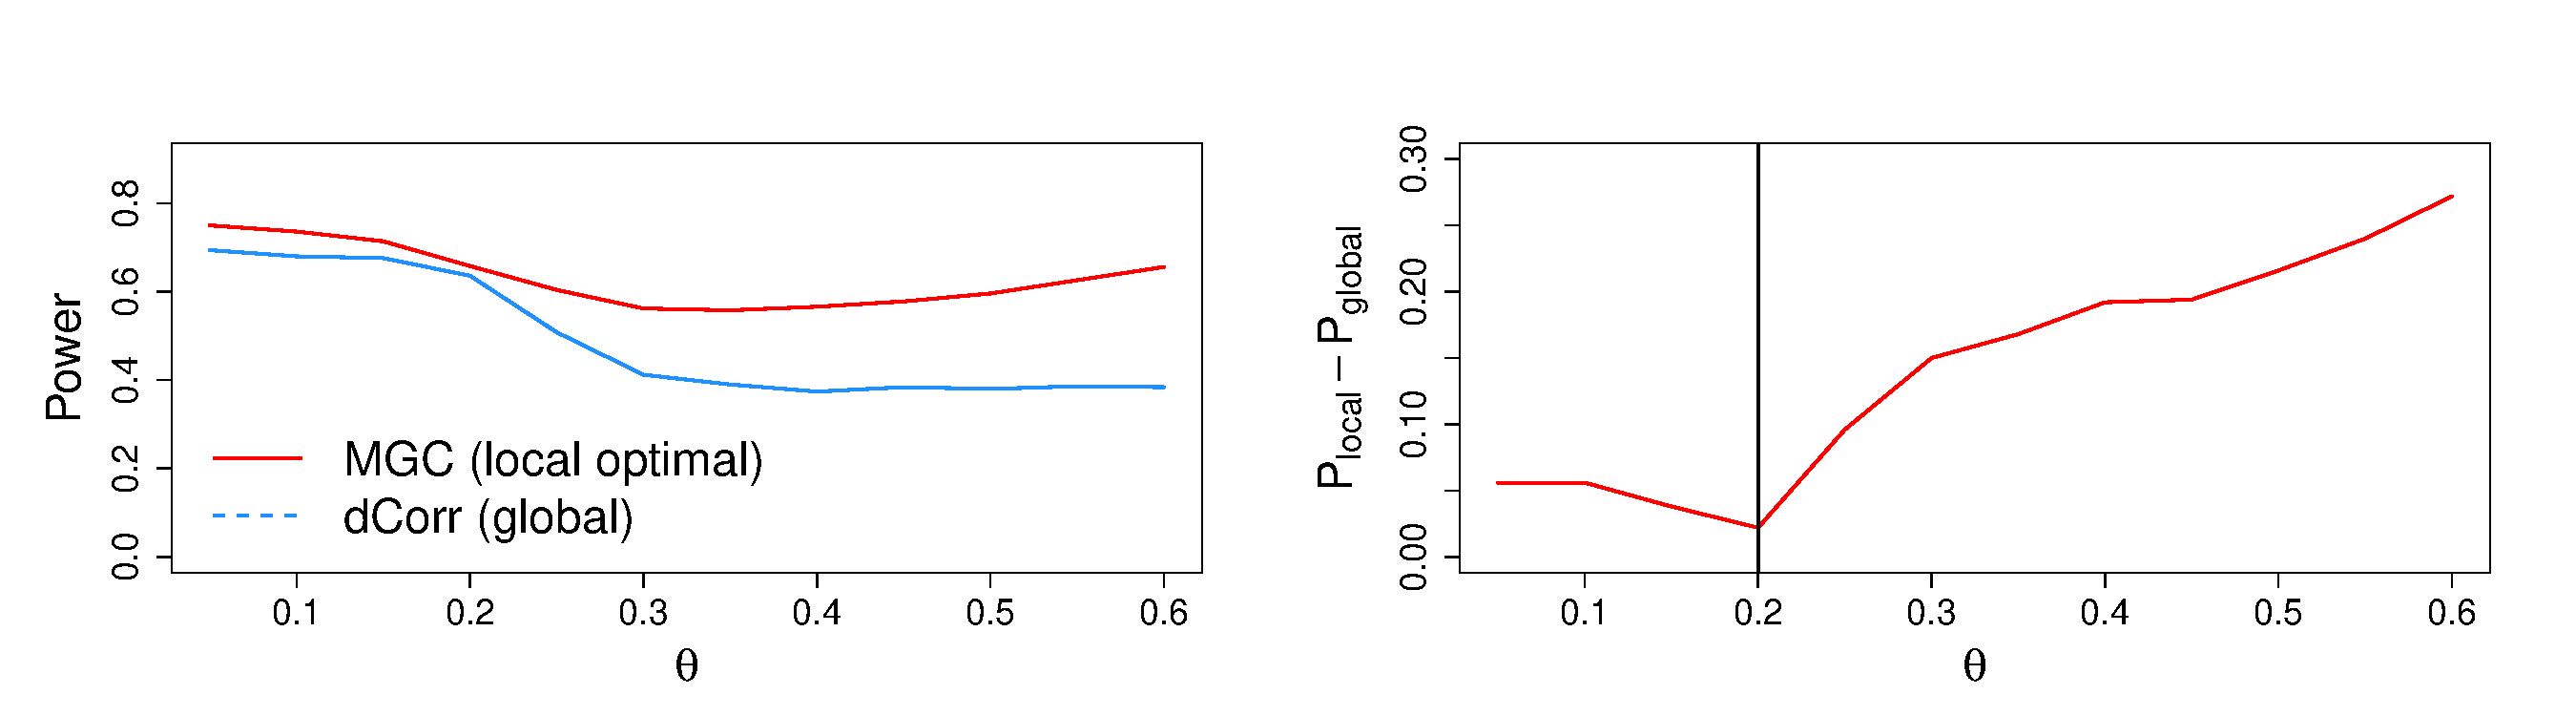
\includegraphics[width=\linewidth]{../../Figure/powerplot_simple.pdf}
	\caption{X-axis of $\theta$ controls the existence/amount of nonlinear dependency and in this particular case nonlinearity exists when $\theta > 0.2$ and gets larger as it increases. You can see the discrepancy in power between global and local scale tests also gets larger accordingly, \textbf{mostly due to decreasing power of global test but relatively stable power of \texttt{MGC} under nonlinear dependency} as presented in the left panel.}
	\label{fig:powerplot}
\end{figure}
If you see Figure~\ref{fig:powerplot}, power of \texttt{dCorr} starts to drop from $\theta = 0.2$ while that of \texttt{MGC} almost stays clam.This implies \texttt{MGC} keeps its sensitivity even under nonlinear dependency compared to \texttt{dCorr}.

\subsection{Degree-corrected two block model}

The SBM connotes that all nodes within the same block have the same expected degree. However the network model of homogeneous distribution within block leads to a poor fit to networks with highly varying node degrees even within block. Out of this concern, the Degree-Corrected Stochastic Block model (DCSBM) varies distribution of node degree within a block, preserving the overall block community structure~\citep{karrer2011stochastic}. Consider two block SBM having more variability induced by $V$ (model~\ref{eq:dcVariance}). Here we have an edge distribution as a linear function of Euclidean distance of $X$. However its variance becomes inflated due to $\tau > 0$. Relatively poor performance of an adjacency metric as presented in Figure~\ref{fig:dcSBM} can be attributed to large variability in it. Even in this case, \texttt{MGC} achieves almost same level of power across increasing $\tau$s. On the other hand, node-specific latent factors look more sensitive in \texttt{FH} model, but still diffusion maps metrics work better.

\begin{figure}[H]
	\centering
		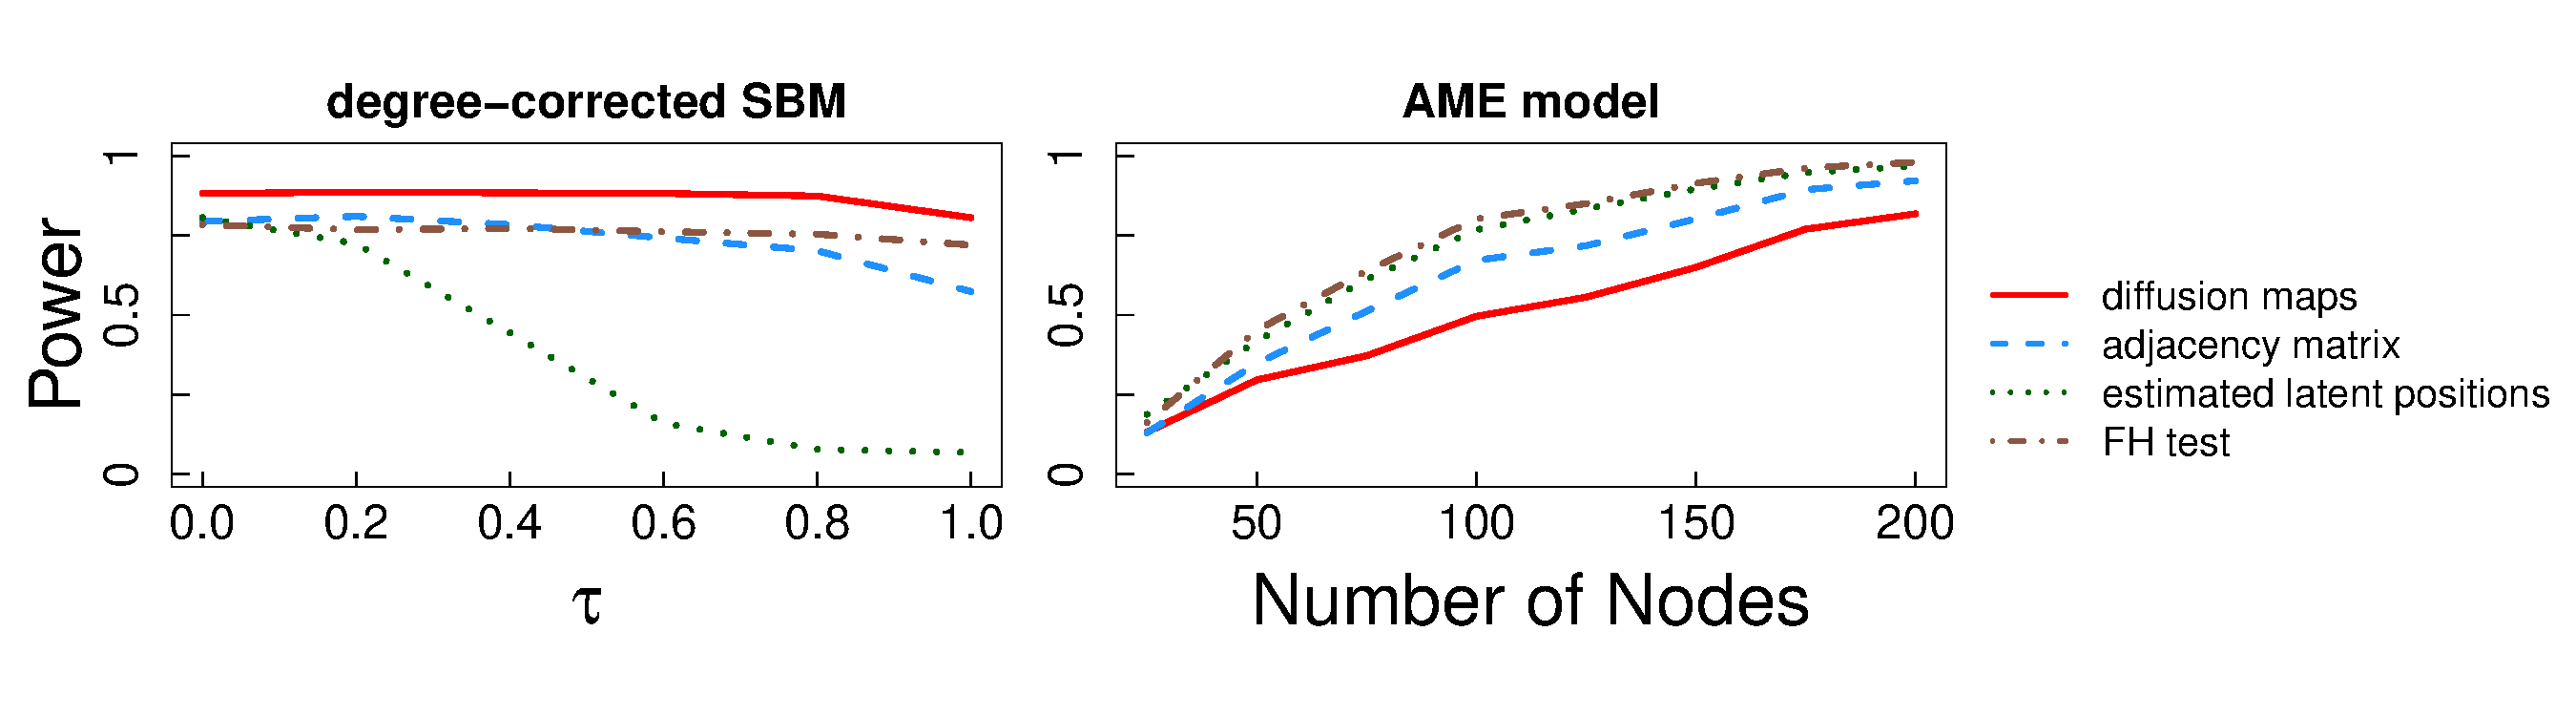
\includegraphics[width=\textwidth]{../../Figure/amedc.pdf}
	\caption{(a) In degree-corrected SBM where the variability in degree distribution increases as $\tau$ increases, testing power of diffusion maps are more likely to be robust against increasing variability compared to other network metrics, e.g. adjacency matrix or latent positions. \texttt{FH} test statistics allowing different dimensions of network factors perform consistently well but still have less power than \texttt{MGC}. (b) \texttt{MGC} utilizing diffusion distances loses some power under additive and multiplicative model which favors estimated latent position metrics, but \texttt{MGC} does as good as \texttt{FH} tests under latent factor metrics which closes to the truth. This reveals the flexibility in distance-based matrix in \texttt{MGC} statistics, which can be chosen depending on model fit or preliminary knowledge.}
	\label{fig:combined}
\end{figure}	
	
\subsection{Additive and multiplicative graph model}
\label{ssec:ame}

\cite{hoff2002latent} proposed an approach of modeling network as an additive and multiplicative function of node-specific latent factors. Whereas \cite{fosdick2015testing} embedded nodes into latent factors assuming that their network model is \textit{correct}, a family of diffusion maps are nonparametric version of embedding nodes into multivariate variable without losing any information on adjacent relationship. Thus in the model~\ref{eq:ame}, where logit of $A$ obeys the presumed model, the estimated latent factors would be very close to the truth, much closer than embedding made from diffusion maps. Even though we rarely see the network nearly follows the model in reality, If we should, using network factors as independent observations from graph \textbf{G} and applying them to \texttt{MGC} performs not very worse than \texttt{FH} statistic (Figure~\ref{fig:ame}). In other words, if network really fits well to the network model with node-specific latent factors as covariates, then it would safe to use those factors in the \texttt{MGC} statistic directly. Since they assume \textit{i.i.d} generative model for factors, there is nothing wrong with applying \texttt{MGC} using \textit{i.i.d} observations of estimated factors.

\subsection{Node Contribution Test}
\label{ssec:node}

\begin{figure}[h]
	\centering
	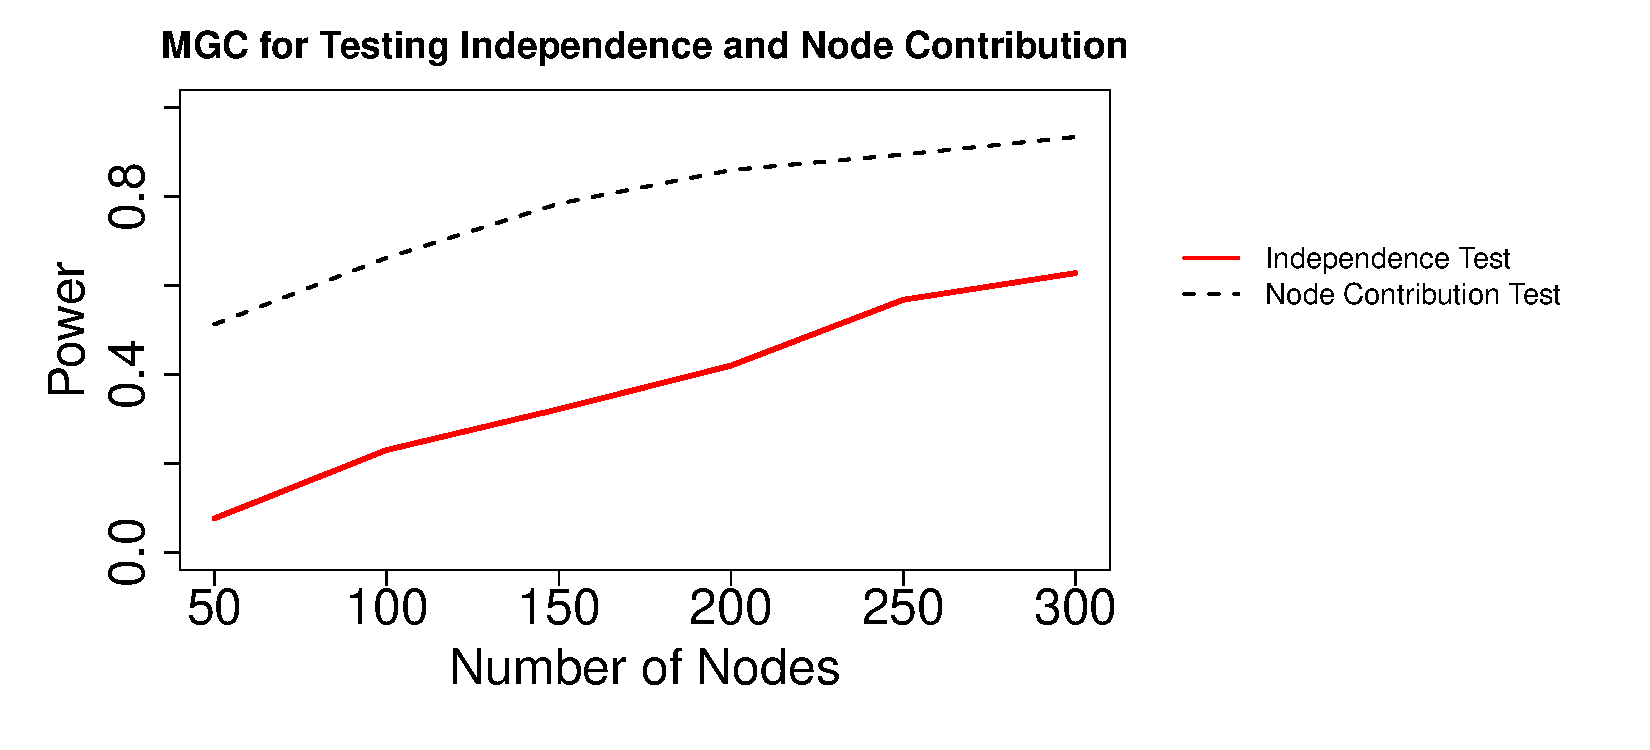
\includegraphics[width=\linewidth]{../../Figure/nodecontri.pdf}
	\caption{This plot describes that both power of \texttt{MGC} and the rate of correctly-ranked node contribution increase as the number of nodes increases when only half of the nodes for each simulation actually are set to be dependent on network, \textbf{which validates the use of node contribution measure in independence test.}}
	\label{fig:contribution}
\end{figure}
To examine the effectiveness of node contribution measure in testing dependency as presented in the statistic~\ref{eq:contribution}, we deliberately simulate the network and its nodal attributes as half of the nodes are independent while the other half are dependent on network (model~\ref{eq:contri}). As an ad hoc test of node contribution, we rank the nodes in terms of decreasing order of $c(v)$ and count the ratio of dependent samples's ranks within the number of dependent nodes. If it works perfectly, all dependent nodes would take higher rank than every independent node so thus the rate equals to one. We call this rate as \textit{inclusion rate}:
\begin{equation}
\mbox{ inclustion rate}\big(  c(v) \big) = \sum\limits_{v \in V(\mathbf{G})} \big\{  rank_{c(v)}\big(  v \big)  \leq  m  \big\}   /  m,
\label{eq:inclusion_rate}
\end{equation}
where $m (\leq |V(\mathbf{G})|)$ is the number of nodes under network dependence. We set $m=n/2$ out of $n = |V(\mathbf{G})|$.

%%%%%%%%%%%%%%%%%%%%%%%%%%%%%%%%%%%%%%%%%%%%%%%%%%%%%%%%%%%%%%%%
\section{Real Data Examples}
\label{sec:real}

\begin{figure}[H]
	\centering
	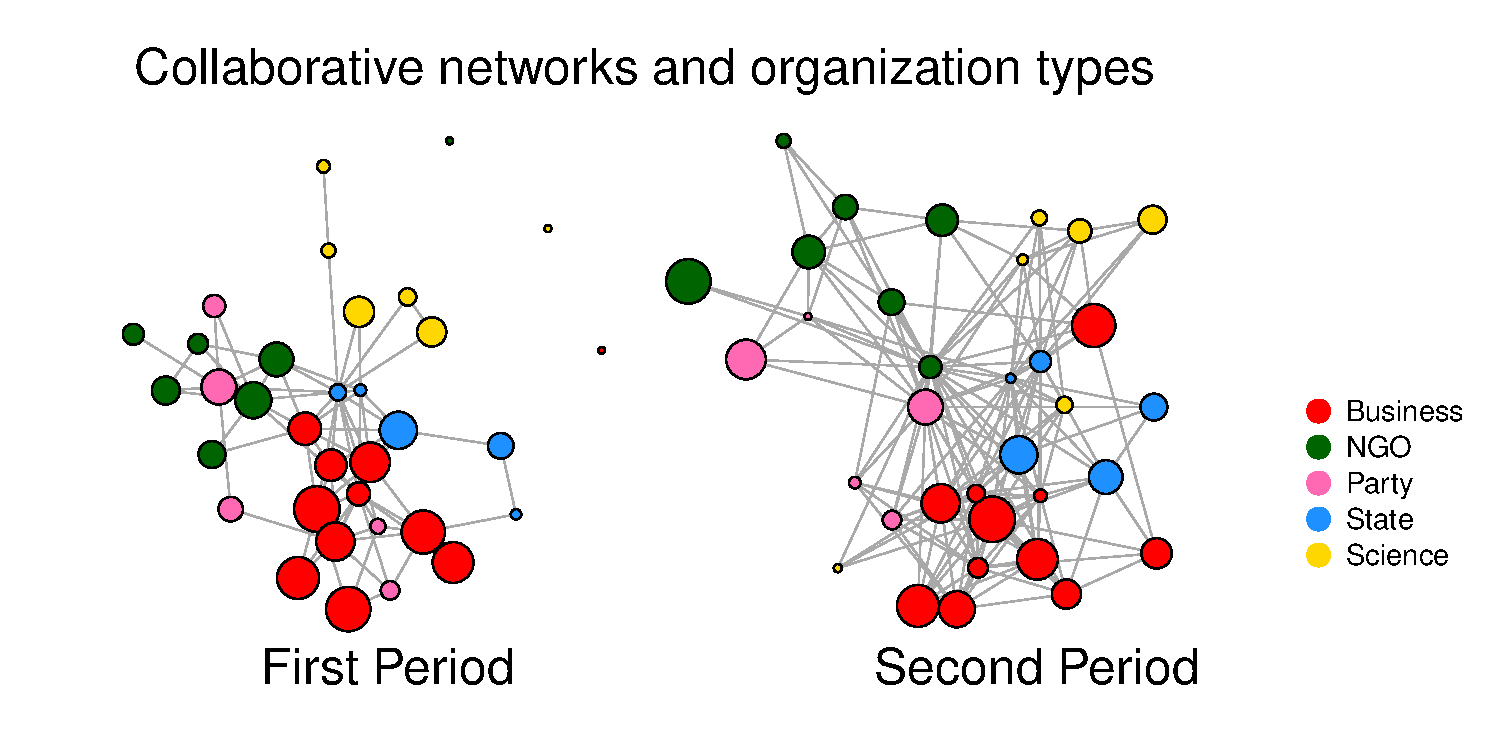
\includegraphics[width=\linewidth]{../../Figure/two_politics.pdf}
	\caption{Both panels depict the collaborative networks during the two time periods having significant network dependency in types of organizations. \textbf{Using \texttt{MGC} statistics, we are not only able to test network independence but also calculate each node's amount of contribution to detecting dependence, which is proportional to node size here.} You can tell that the tendency to collaborate within the same type is strongest among the business group while scientist relatively collaborates less with any others, especially in the first period.}
	\label{fig:politics}
\end{figure}
	
In the field of political science, who exerts more powerful impacts than others over political network and which factors impact on the power differentials are one of the interests~\citep{ingold2014structural}. \cite{minhas2016inferential} made an inference from political networks~\citep{cranmer2016navigating} via the additive and multiplicative effects (AME). As mentioned in Section~\ref{ssec:ame}, the AME model estimates the latent factors and uses them to test independence with the nodal attributes. Among diverse attributes that \cite{cranmer2016navigating} provided, we focus on the types of organizations and how 34 political organizations having different types are participating policy network. We changed a given directed network into undirected network and use a dissimilarity matrix for distance matrix of the attributes, i.e., $\parallel \mathbf{X}_{i}  - \mathbf{X}_{j} \parallel = 0$ if and only if node $i$ and node $j$ are from the same type and one otherwise. Two collaboration networks comprised of the same set of nodes across two time periods are provided~\citep{ingold2014structural}. Figure~\ref{fig:politics} and Figure~\ref{fig:barplots} illustrates these two networks and shows each node's reliance on its organization type when collaborating. For two periods, the network independence test statistics of \texttt{MGC} and \texttt{dCorr} using diffusion distance matrices result in significant p-values across diffusion times from $t=1$ to $t=10$. The conclusion from the \texttt{FH} test is also the same.  

\begin{figure}[h]
	\centering
	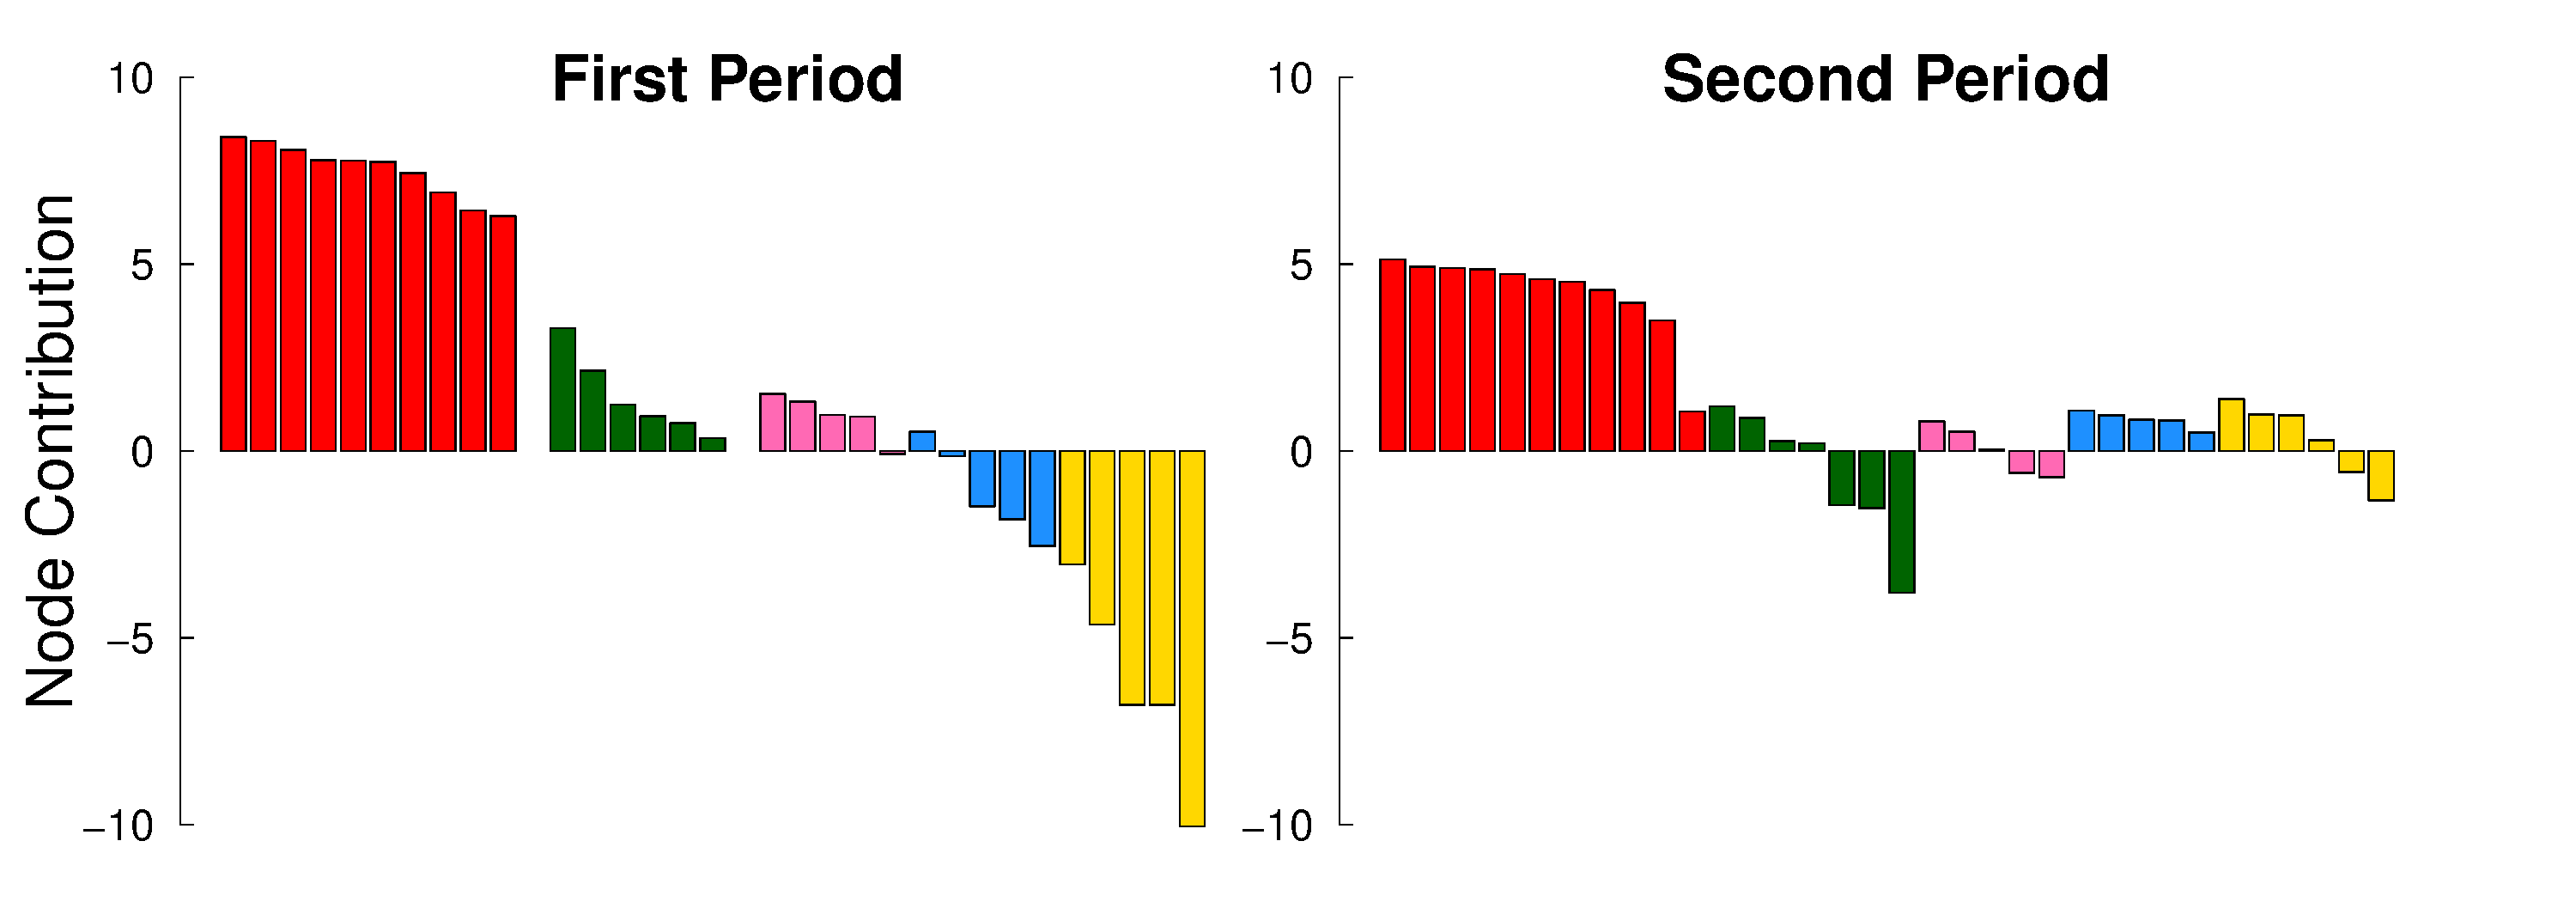
\includegraphics[width=\linewidth]{../../Figure/barplots_nolegend.pdf}	
	\caption{In the first period, we have two extreme cases among the business group and science group, which reflects our observations in Figure~\ref{fig:politics}. Generally organizations cooperate more actively between different types in the second period but still their collaboration network is highly dependent on their organization types.}
	\label{fig:barplots}
\end{figure}

%%%%%%%%%%%%%%%%%%%%%%%%%%%%%%%%%%%%%%%%%%%%%%%%%%%%%%%%%%%%%%%%
\section{Discussions}
\label{sec:discussion}
	
In this paper, we have shown that \texttt{MGC}, merged with a family of diffusion distance, provides us powerful independence test statistics in network. Having multiscale statistics, i.e. one parameter family of statistics, is not avoidable because \textbf{we regard distance between nodes over network as a dynamic process.} Through simulation studies, we demonstrated that our methods work better that the others especially under nonlinear dependency, and we are able to measure each node's contribution to detecting dependence. Deriving the contributions is particularly important in nonlinear network dependence since we assume possibly different amount of the dependencies among the nodes.  

However obtaining a full family of statistics are computationally infeasible. Also we did not suggest any theoretically supported tools to select one metrics among them so thus we have one single statistic. As an ad hoc, we selected an \textit{optimal} diffusion time $t$ with highest power from $t=1$ to $t=10$ for our simulation since we could observe a stabilized empirical power within this period. In the real data study we have significant p-values across diffusion time $t=1$ to $t=10$. 
\textbf{Developing the adaptive method to find this optimal $t$ when dependence is maximized would be a natural next step.} Despite these shortcomings, a range of applications based on our work are very diverse. Even though we specifically constraint the statistic into testing independence between network and nodal attributes, \textbf{we are able to implement independence testing between two networks of same size by using diffusion distance of each network.} This type of test will be useful when we want to investigate whether a pair of networks are topologically or structurally independent. In this possible extension, we could also enjoy both \texttt{MGC} and a family of diffusion distances which are specialized in preserving local relationship between the two data sets. 

%%%%%%%%%%%%%%%%%%%%%%%%%%%%%%%%%%%%%%%%%%%%%%%%%%%%%%%%
\appendix
\section{appendix}
\label{sec:appendix}

\subsection{simulation schemes}
\begin{itemize}	

	\item \textbf{Three Block SBM}
	\begin{equation}
	\label{eq:Three}
	\begin{gathered}
	\begin{aligned}
	&  X_{i} \overset{i.i.d}{\sim} f_{X}(x)   \stackrel{d}{=}  Multi(1/3, 1/3, 1/3), \quad i = 1, \ldots , n \\ 
	&  Z_{i} | X_{i}  \overset{i.i.d}{\sim}    f_{Z|X}(z|x)  \stackrel{d}{=}   Multi(0.5, 0.25, 0.25) I( x = 1 ) +   Multi(0.25, 0.5, 0.25) I (x = 2)  \qquad  \\ & \quad \quad + Multi(0.25, 0.25, 0.5)I(x = 3), \quad  i = 1,\ldots,n  \\
	&  A_{ij} | Z_{i}, Z_{j}   \overset{i.i.d}{\sim}   f_{A|Z}(a_{ij} | z_{i}, z_{j}) \stackrel{d}{=}  Bern(0.5) I ( |z_{i} - z_{j}| = 0 )  + Bern(0.2) I(|z_{i} - z_{j}| = 1) \\ & \quad \quad + Bern(0.3) I (|z_{i} - z_{j}| = 2),  \quad i,j=1, \ldots n ; \quad i < j.
	\end{aligned}
	\end{gathered}
	\end{equation}
	
\item \textbf{Increasing variance in DCSBM}
	\begin{equation}
	\label{eq:dcVariance}
	\begin{gathered}
	\begin{aligned}
	&  X_{i} \overset{i.i.d}{\sim} f_{X}(x)   \stackrel{d}{=}  Bern(0.5), \quad i = 1, \ldots , n \\ 
	&  Z_{i} | X_{i}  \overset{i.i.d}{\sim}    f_{Z|X}(z|x)  \stackrel{d}{=}   Bern(0.6) I( x = 0 ) +   Bern(0.4) I (x = 1), \quad  i = 1,\ldots,n  \\
	& V_{i} \overset{i.i.d}{\sim} Uniform(1 - \tau, 1 + \tau),\quad i = 1, \ldots, n; \quad \tau = 0, 0.2, \ldots, 1\\ 
	& A_{ij} | Z_{i}, Z_{j}, V_{i}, V_{j}   \overset{i.i.d}{\sim}   f_{A|Z, V}(a_{ij} | z_{i}, z_{j}, v_{i}, v_{j}) \stackrel{d}{=} Bern(0.2 \cdot v_{i} v_{j}) I ( |z_{i} - z_{j}| = 0 ) \\ & \quad \quad + Bern(0.05 \cdot v_{i} v_{j} ) I(|z_{i} - z_{j}| = 1), \quad i,j=1, \ldots, n; i < j. 
	\end{aligned}
	\end{gathered}
	\end{equation}

\item \textbf{Additive and Multiplicative Graph Model}
\begin{equation}
	\label{eq:ame}
	\begin{gathered}
	\begin{aligned}
	&	Z_{i} \overset{i.i.d}{\sim} f_{Z}(z) \stackrel{d}{=} Uniform[0,1]. \quad i = 1, \ldots, n \\ 
	&	X_{i} | Z_{i} \overset{i.i.d}{\sim}  f_{X|Z}(x|z) \stackrel{d}{=}  Normal(Z_{i}, 1), \quad i= 1, \ldots, n \\
	&	A_{ij} | Z_{i}, Z_{j} \overset{i.i.d}{\sim}  f_{A|Z}(a_{ij} | z_{i}, z_{j}) \stackrel{d}{=}   Bern \big(  ( 1 - z_{i})^2 \times (1 - z_{j})^2    \big), \quad i,j = 1, \ldots, n; i < j.
	\end{aligned}
	\end{gathered}
\end{equation}	

\item \textbf{Node Contribution}
\begin{equation}
\begin{gathered}
\begin{aligned}
& X_{i} \overset{i.i.d}{\sim} f_{X}(x)   \stackrel{d}{=}  Bern(0.5)  \quad i = 1, \ldots ,n/2, \ldots, n \\ & Z_{i} | X_{i}  \overset{i.i.d}{\sim}    f_{Z|X}(z|x)  \stackrel{d}{=}   Bern(0.6) I(x = 0) + Bern(0.4) I(x=1), \quad  i = 1,\ldots,n/2, \ldots, n \\
& A_{ij} | Z_{i}, Z_{j}   \overset{i.i.d}{\sim}   f_{A|Z}(a_{ij} | z_{i}, z_{j})  \\ & \quad  \quad \stackrel{d}{=} \left\{  \begin{array}{cc} Bern(0.4) I(|z_{i} - z_{j}| = 0)  + Bern(0.1) I(|z_{i} - z_{j}| > 0) & i = 1,\ldots,n/2 \\   Bern(0.25)  & i=1+n/2, \ldots, n  \end{array} \right.
\end{aligned}
\end{gathered}
\label{eq:contri}
\end{equation}

\end{itemize}


%%%%%%%%%%%%%%%%%%%%%%%%%%%%%%%%%%%%%%%%%%%%%
\subsection{Algorithms}
\alglanguage{pseudocode}

\begin{algorithm}[H]
	\caption{Mutiscale representation of nodes in network}
	\begin{algorithmic}[1]
		\Require Transition probability matrix $P$ of network $G$ and a set of time points $\{ t_{i}  : t_{i} \in \mathbb{N} \}$  of diffusion time. 
		\Ensure A list of diffusion maps at each time point.
		\Function{ \texttt{dmap} }{ $n \times n$ transition matrix $P$, time points $\{ t_{1}, t_{2}, \ldots, t_{K} \}$ } 
		\State $\mathbf{\pi} :=$ \texttt{statdistr}($P$)\Comment{stationary distribution of $P$} 
		\State $\Pi : =$ \texttt{Diag}($\mathbf{\pi}$)\Comment{Diagonal matrix with diagonal element of $\mathbf{\pi}$}
		\State $Q: = \Pi^{1/2} P \Pi^{-1/2}$ 
		\State $\lambda := $ \texttt{eigenvalue}($Q$)\Comment{a real-valued vector with length of $q (\leq n)$. }
		\State $\Lambda : =$ \texttt{Diag}($\lambda$)
		\State $\Psi : =$ \texttt{eigenfunction}($Q$)\Comment{$n \times q$ real-valued matrix} 
		\State $\Phi :=  \Pi^{-1/2} \Psi$\Comment{$n \times q$ real-valued eigenfunction matrix of $P$}
		\For{$t_{i}$ :  $i$ = 1 }{ $K$}
		\Begin
		\State \texttt{Maps}$[i] := \Phi \Lambda^{t_{i}}$  
		\End
		\EndFor
		\State \texttt{Maps} = list( \texttt{Maps}[1], \texttt{Maps}[2], $\ldots$, \texttt{Maps}[$K$]  )
		
		\Return \texttt{Maps}
		\EndFunction
	\end{algorithmic}
\end{algorithm}

%%%%%%%%%%%%%%%%%%%%
\begin{algorithm}[H]
	\caption{Multiscale Generalized Correlation (\texttt{MGC}) test statistics with diffusion maps as a network-based distance.}
	\begin{algorithmic}[1]
		\Require A connected, undirected network $G$ with its nodal attributes $\mathbf{X}$.
		\Ensure A list of \big(  (a) p-value of \texttt{sample MGC}, (b) estimated \texttt{sample MGC} statistic, (c) p-value map for all local correlations, (d) a set of estimated optimal neighborhood scales $\{  (k^{*}, l^{*}  ) \}$  \big) for each diffusion maps.
		\Function{ \texttt{NetworkTest} }{ $G$, $\textbf{X}$,  $\mathbf{T}$ := (diffusion time points $\{ t_{1}, t_{2}, \ldots, t_{K} \}$)  }
		\State $A :=$ \texttt{get.adjacency}$(G)$\Comment{obtain an adjacency matrix of network $G$}
		\State $P := A $ / \texttt{rowSums}($A$) 
		\State $U :=$ \texttt{dmap}($P$, $\mathbf{T}$) \Comment{a list of diffusion maps in each time point}
		\For{$t_{i}$ :  $i$ = 1 }{ $K$}
		\Begin
		\State $C : =$  \texttt{dist}($U[i]$) \Comment{distance matrix of diffusion maps at time $t_{i}$}
		\State $D : =$ \texttt{dist}($X$) \Comment{distance matrix of nodal attributes}
		\State \texttt{MGC}$[i]$ = \texttt{MGCPermutationTest}( $C$, $D$ ) 
		\End
		\EndFor
		\State \texttt{MGC} = list( \texttt{MGC}[1], \texttt{MGC}[2], $\ldots$, \texttt{MGC}[$K$]  )
		
		\Return \texttt{MGC}
		\EndFunction
	\end{algorithmic}
\end{algorithm}

%%%%%%%%%%%%%%%%%%%%%%
\begin{algorithm}[H]
	\caption{Node-specific contribution to detecting dependency via \texttt{MGC} statistic}
	\begin{algorithmic}[1]
		\Require Distance metric of graph $G$, $C$, and attributes $X$, $D$, and (one of) the estimated optimal scales $\{ k^{*}, l^{*} \}$ 
		\Ensure  unstandardized contributions of each node in network $\{  c(v) \}$
		\Function{ \texttt{Contribution} }{   C, D , $\{  (k^{*}, l^{*}) \}$   }
		\State $\tilde{C} : = \texttt{DoubleCentering}(C)$
		\State $\tilde{D} := \texttt{DoubleCentering}(D)$
		\State \texttt{Rank}($M_{ij}$):= (rank of node $j$ with respect to node $i$)
		\For{$v = 1$}{ $|V(G)|$} \Comment{iterate over every each node}
		\State $c(v) = 0$
		\For{$j = 1$}{ $n$}
		\Begin
		\State $c(v) =  c(v) + \tilde{C}_{vj} \tilde{D}_{v j} I(  \texttt{Rank}(C_{vj})  \leq k^{*}, \texttt{Rank}(D_{vj}) \leq l^{*} )$
		\End
		\EndFor
		\EndFor
		\State \texttt{cset} $:= \{ c(v) : v = 1,2, \ldots , |V(G)|  \}$	
		
		\Return  \texttt{cset}
		\EndFunction
	\end{algorithmic}
\end{algorithm}

%%%%%%%%%%%%%%%%%%%%%%%%%%%%%%%%%%%%%%%%%%%%%	
\newpage
\subsection{Lemmas and Theorems}
	
\begin{theorem}[\textit{de Finetti's Theorem}] 
\label{finetti}	
\bigskip			
Let $\mathbf{X}_{1}, \mathbf{X}_{2}, ...$ be an infinite sequence of random variables with values in a space of $\mathbf{X}$. The sequence $\mathbf{X}_{1}, \mathbf{X}_{2}, ...$ is exchangeable \textit{if and only if} there is a random probability measure $\eta$ on $\mathbf{X}$ such that the $X_{i}$ are conditionally i.i.d. given $\eta$. 
\end{theorem}
	
\begin{theorem}[\textit{Aldous Hoover Theorem}]
		\label{Aldous_Hoover}
		
Let $\mathbf{A} = \{A_{ij}\}, 1 \leq i,j \leq \infty$ be a jointly exchangeable binary array if and only if there exists a random measurable function $f : [0,1]^{3} \rightarrow \mathbf{A}$ such that 
		
\begin{equation}
	\big(  A_{ij}  \big) \stackrel{d}{=} \left( f \big( U_{i}, U_{j}, U_{ij} \big)  \right),
\end{equation}
		where $(U_{i})_{i \in \mathbb{N}}$ and $(U_{ij})_{i,j > i \in \mathbb{N}}$ with $U_{ij} = U_{ji}$ are a sequence and matrix, respectively, of \textit{i.i.d} Uniform[0,1] random variables. 
\end{theorem}
	
%%%%%%%%%%%%%%%%%%%%%%%%%%%%%%%%%%%%%%%%%%%%
\begin{proof}[\textbf{Proof of spectral decomposition of diffusion distance}]
	Diffusion distance of $\mathbf{G}$ can be represented via a spectral decomposition of its transition matrix $P$~\citep{coifman2006diffusion,lafon2006diffusion}. Recall that diffusion distance at time $t$, $C_{t}$, is a functional $L^2$ distance, weighted by 1/$\pi$ in the statistic~\ref{eq:diffusion}. Since an adjacency matrix $A$ does not guarantee a symmetry of $P$, define a symmetric kernel $Q = \Pi^{1/2} P \Pi^{-1/2}$, where $\Pi$ is a $n \times n$ diagonal matrix of which $i$th diagonal element is $\pi(i)$. Under compactness of $P$, $Q$ has a discrete set of real nonzero eigenvalues $\{ \lambda_{r} \}_{r = \{1,2,...,q \}}$ and a set of their corresponding orthonormal eigenvectors $\{ \psi_{r} \}_{r = \{1,2,..., q \} },$ i.e. $Q[i,j] = \sum\limits_{r=1}^{q} \lambda_{r} \psi_{r}(i) \psi_{r}(j)$ ($1 \leq q \leq n$). Returning to the transition probability between Node $i$ and Node $j$,
	
	\begin{equation}
	\begin{split}
	P[i,j] &  = \sqrt{\pi(j) / \pi(i) } Q[i,j] \\ &   = \sum\limits_{r=1}^{q} \lambda_{r} \big\{ \psi_{r}(i) / \sqrt{\pi(i)}  \big\} \big\{ \psi_{r}(j) \sqrt{\pi(j)} \big\}  \\ & : = \sum\limits_{r=1}^{q} \lambda_{r} \phi_{r}(i) \big\{ \psi_{r}(j) \sqrt{\pi(j)} \big\}
	\end{split}
	\end{equation}
	where $\phi_{r}(i) := \psi_{r}(i) / \sqrt{\pi(i)}$. Since $\sum\limits_{r=1}^{q} \psi^2_{r}(j) = 1$ for all $j \in \{1,2,...,n\}$, we can represent the diffusion distance at time $t$ as: 	
	\begin{equation}
	\begin{split}
	C^2_{t}[i,j]  = \sum\limits_{r=1}^{n} \lambda^{2t}_{r} \big( \phi_{r} (i) - \phi_{r}(j)   \big)^2  
	\end{split}
	\end{equation}
	That is,
	\begin{equation}
	C_{t}[i,j] = \parallel \mathbf{U}_{t}(i) - \mathbf{U}_{t}(j) \parallel
	\end{equation}
	where 
	\begin{equation} 
	\mathbf{U}_{t}(i) = \begin{pmatrix} \lambda^{t}_{1} \phi_{1}(i) & \lambda^{t}_{2} \phi_{2} (i)  & \ldots & \lambda^{t}_{q} \phi_{q}(i) \end{pmatrix}^{T} \in \mathbb{R}^{q}.
	\end{equation}
	
\end{proof}	
	
%%%%%%%%%%%%%%%%%%%%%%%%%%%%%%%%%%%%%%%%%%%%%%%%%		
\begin{proof}[\textbf{Proof of Lemma~\ref{lemma_graphon} }] 
	By \textit{Aldous-Hoover Theorem}~\ref{Aldous_Hoover}, a random array $(A_{ij})$ is jointly exchangeable \textit{if and only if} it can be represented as follows : 
		
	There is a random function $g : [0,1]^2 \rightarrow [0,1]$ such that 
\begin{equation}
(A_{ij})  \stackrel{d}{=} Bern( g(W_{i}, W_{j})), \quad i,j=1,\ldots,n; i < j
\end{equation}
where $W_{i} \overset{i.i.d.}{\sim} Uniform(0,1)$. Thus if $\mathbf{A}$ is an adjacency matrix of an undirected, exchangeable network, for any $i,j = 1,... , n; i < j$:
\begin{equation}
\begin{split}
	f_{A} \big(  a_{ij} \big) & = \int f_{A} \big( a_{ij} \big| w_{i}, w_{j} \big) f_{W}(w_{i}) f_{W}(w_{j}) dw dw \\ & = \int_{0}^{1} \int_{0}^{1} g( w_{i},  w_{j})^{a_{ij}} \big( 1- g( w_{i},  w_{j}) \big)^{1-a_{ij}} dw_{i} dw_{j} 
\end{split}
\end{equation}
		
Then within each row, adjacent elements are independent and also identically distributed except a diagonal element.

\end{proof}
		
%%%%%%%%%%%%%%%%%%%%%%%%%%%%%%%%%%%%%%%%	
\begin{proof}[\textbf{Proof of Lemma~\ref{main_lemma}}]
We have shown that for fixed time $t$, diffusion distance is defined as an Euclidean distance of diffusion maps. Diffusion map at time $t$ is represented as follows :
\begin{equation}
	\mathbf{U}_{t}(i) = \begin{pmatrix} \lambda^{t}_{1} \phi_{1}(i) & \lambda^{t}_{2} \phi_{2} (i)  & \cdots & \lambda^{t}_{q} \phi_{q}(i) \end{pmatrix} \in \mathbb{R}^{q}.
\end{equation}
where $\Phi = \Pi^{-1/2}\Psi$ and $Q= \Psi \Lambda \Psi^{T} = \Pi^{1/2} P \Pi^{-1/2}$. 
Thus $P \Pi^{-1/2} \Psi = \Pi^{-1/2} \Psi \Lambda$. 
Then for any $r$th row ($r \in \{1,2, ... , q \}$, $(q \leq n)$), we can see that $P \phi_{r} = \lambda_{r} \phi_{r}$  where $\phi_{r} = \begin{pmatrix}  \psi_{r}(1) / \sqrt{\pi(1)} &  \psi_{r}(2) /  \sqrt{\pi(2)} & \cdots & \psi_{r}(n) /  \sqrt{\pi(n)}  \end{pmatrix}$.
Therefore to guarantee exchangeability (or \textit{i.i.d}) of $\mathbf{U}_{t}$, it suffices to show exchangeability (or \textit{i.i.d}) of $P$.

Assume joint exchangeability of $\mathbf{G}$, i.e. $(A_{ij}) \stackrel{d}{=} \big( A_{\sigma(i) \sigma(j)} \big)$. Since $A_{ij}$ is binary, $A_{ij} / \sum\limits_{j} A_{ij} = A_{ij} /  (1 + \sum\limits_{l \neq j} A_{il})$. Moreover, $A_{ij}$ and $(1 + \sum\limits_{l \neq j} A_{il})$ are independent given its link function $g$, and $A_{\sigma(i) \sigma(j)}$ and $(1 + \sum\limits_{l \neq j} A_{\sigma(i) \sigma(l)})$ are independent also given $g$.
Then the following joint exchangeability of transition probability holds for $i \neq j; i,j = 1,2, \ldots,n$:

\begin{equation}
\big( P_{ij} \big) = \left(  \frac{A_{ij}}{1 - A_{ij} + \sum\limits_{j=1}^{n} A_{ij} } \right)  \stackrel{d}{=} \left( \frac{A_{\sigma(i) \sigma(j)} }{1 - A_{\sigma(i) \sigma(j)} + \sum\limits_{\sigma(j) = 1}^{n} A_{\sigma(i) \sigma(j)} } \right) = \big( P_{\sigma(i) \sigma(j)} \big)
\end{equation}
		
When $i = j$, $P_{ij} = P_{\sigma(i) \sigma(j)} = 0$ for $i=1,2, \ldots, n$. Thus, transition probability is also exchangeable. This results exchangeable eigenfunctions $\{ \Phi(1), \Phi(2), , ... , \Phi(n) \}$ where $\Phi(i) := \begin{pmatrix} \phi_{1}(i) & \phi_{2}(i) & \cdots & \phi_{q}(i) \end{pmatrix}^{T}$, $i=1,2, \ldots, n$. Thus diffusion maps at fixed $t$, $\mathbf{U}_{t} = \begin{pmatrix} \Lambda^{t} \Phi(1)  & \Lambda^{t} \Phi(2) & \cdots & \Lambda^{t} \Phi(n)  \end{pmatrix}$ are exchangeable. Furthermore by \textit{de Finetti's Theorem}~\ref{finetti}, we can say that $\mathbf{U}(t) = \{ \mathbf{U}_{t}(1), \mathbf{U}_{t}(2), \ldots, \mathbf{U}_{t}(n)    \}$ are conditionally independent on their underlying distribution.
\end{proof}
	
%%%%%%%%%%%%%%%%%%%%%%%%%%%%%%%%%%%%%%%%%%%	
\begin{proof}[\textbf{Proof of Lemma~\ref{lemma_graphex}}]
	Based on Kallenberg and Exchangeable Graph (KEG) frameworks, introduced in \cite{veitch2015class}, a random array $(A_{ij})$ is jointly exchangeable in terms of Poisson process \textit{if and only if} it can be represented as follows : there is a random function $g : \mathbb{R}^{2}_{+} \rightarrow [0,1]$ such that 
	
	\begin{equation}
	(A_{ij})  \stackrel{d}{=} (A_{v_{i}, v_{j}} )  \stackrel{d}{=} Bern( g( \vartheta_{i}, \vartheta_{j})), \quad i,j=1,\ldots,n ;\quad i < j,
	\end{equation}
	where $v_{i} \overset{i.i.d.}{\sim} Poisson(1), \vartheta_{i} \overset{i.i.d.}{\sim} Poisson(1), v_{i} \leq \nu$, for some pre-specified $\nu >0$ so that finite-sized graph can deliberately include nodes only if they participate in at least one edges. Thus if $\mathbf{A}$ is an adjacency matrix of such undirected, exchangeable network, for any $i,j = 1,... , n; i < j$:
\begin{equation}
\begin{split}
	f_{A | V} \big( a_{ij} \big| v_{i}, v_{j} \big) & = \int f_{A | V, \vartheta} \big( a_{ij} \big| v_{i}, v_{j}, \vartheta_{i}, \vartheta_{j} \big) f_{\vartheta} ( \vartheta_{i}) f_{\vartheta}(\vartheta_{j})   d\vartheta_{i} d\vartheta_{j}   \\ & = \int_{0}^{\nu} \int_{0}^{\nu}   g( \vartheta_{i},  \vartheta_{j})^{a_{ij}} \big( 1- g( \vartheta_{i},  \vartheta_{j}) \big)^{1-a_{ij}}  \cdot dPois_{1}(\vartheta_{i}) \cdot dPois_{1}(\vartheta_{j})  d \vartheta_{i} d \vartheta_{j}.
\end{split}
\end{equation}
where $dPois_{1}(\cdot)$ is a probability distribution function of Poisson process with rate of 1.  Thus given $\{ \mathbf{V} \}$, edge probability except self-loop within each row (or column) is conditionally $\textit{i.i.d}$ given a link function $g$ and Poisson process $V$.
\end{proof}
%%%%%%%%%%%%%%%%%%%%%%%%%%%%%%%%%%%%%%%%%%%%%%%%
\begin{proof}[\textbf{Proof of Lemma~\ref{lemma1}} Convergence of empirical characteristic functions of exchangeable variables] 
	
This follows exactly the same as \textit{Theorem 1} in \cite{szekely2007measuring}. Note that this Lemma always holds without any assumption on $\{(\mathbf{w}_{i},\mathbf{y}_{j}), i=1,2,...,n\}$, e.g., it holds without assuming exchangeability, nor identically distributed, nor finite second moments.
\end{proof}

\begin{proof}[\textbf{Proof of Lemma~\ref{lemma2}} Empirical characteristic function of exchangeable variables] 
\bigskip	
It suffices to prove the first argument~\ref{eq:conv1} since the second argument~\ref{eq:conv2} immediately follows from the first one by the property of characteristic functions.
Proving the first one is equivalent to \textit{Theorem 2} in \cite{szekely2007measuring}. However, they required $\{(\mathbf{w}_{i},\mathbf{y}_{i})\}$ to be independently identically distributed as $(\mathbf{w},\mathbf{y})$ with finite second moments; here we have exchangeable $\{ ( \mathbf{w}_{i}, \mathbf{y}_{i}  ) \}$ instead. 

Followed by \textit{de Finetti's Theorem}~\ref{finetti}, if and only if $\{ w_{i} \}$ are (infinitely) exchangeable, there exists an underlying distribution $f_{\mathbf{w}}$ of $\mathbf{w}$ such that $\mathbf{w}_{i}  \overset{i.i.d}{\sim} f_{\mathbf{w}} $. By the same logic there exists a random, we have an underlying distribution $f_{\mathbf{y}}$ where $\mathbf{y}_{i} \overset{i.i.d}{\sim} f_{\mathbf{y}}$. Let $(\mathbf{w}_{i}, \mathbf{y}_{i}) \overset{i.i.d}{\sim}   f_{\mathbf{w}, \mathbf{y}}$. Then under the assumption of finite second moment of the underlying distributions and measurable, conditioned random functions, we have a strong large number for V-statistics followed by \cite{szekely2007measuring}, i.e., 
\begin{eqnarray}
		\displaystyle\int_{D(\delta)}{\|g_{\mathbf{w},\mathbf{y}}^{n}(t,s)-g_{\mathbf{w}}^{n}(t)g_{\mathbf{y}}^{n}(s)\|^{2}}dh &\stackrel{n \rightarrow \infty}{\longrightarrow} 
		 \displaystyle\int_{D(\delta)}{\|g_{\mathbf{w},\mathbf{y}}(t,s)-g_{\mathbf{w}}(t)g_{\mathbf{y}}(s)\|^{2}}dh,
\label{eq:SLLN}
\end{eqnarray}
where $D(\delta)=\{(t,s):\delta \leq |t|_{p} \leq 1/\delta,\delta \leq |s|_{q} \leq 1/\delta\}$, and $h(t,s)$ is the weight function chosen in \cite{szekely2007measuring}. 
\end{proof}

%%%%%%%%%%%%%%%%%%%%%%%
\begin{proof}[\textbf{Proof of Theorem~\ref{theoremMain}} Consistency of \texttt{dCorr} applied to exchangeable variables]
\bigskip
Under the exchangeability and finite moments assumptions of underlying distribution, it follows from Lemma~\ref{lemma1} and \ref{lemma2} that $\mathcal{V}^{2}_{n}(\mathbf{W},\mathbf{Y}) \xrightarrow{n \rightarrow \infty}  0$ if and only if underlying distribution of $\{\mathbf{w}_{i} \}$, $\mathbf{w}$ is independent from underlying distribution of $\{ \mathbf{y}_{i}  \}$, $\mathbf{y}$. Therefore, the \texttt{dCorr} or \texttt{mCorr} converges to $0$ if and only if  underlying distributions are independent; and its testing power converges to $1$ under any joint distribution of finite moments. Since the multiscale generalized correlation based on any consistent global correlation is also consistent~\citep{shen2016discovering}, \texttt{MGC} statistic constructed by \texttt{dCorr} or \texttt{mCorr} is also consistent in testing dependence.
\end{proof}

\begin{proof}[\textbf{Proof of Theorem~\ref{theorem2}} Consistency of \texttt{MGC} applied to exchangeable variables]

Suppose that we have undirected, connected network $\mathbf{G}$ having a family of diffusion maps $\{ \mathbf{u}_{t}(i) : i = 1, \ldots , n ; ~t \in \mathbb{N} \}$ and with nodal attributes $\{ \mathbf{x}_{i} :  i = 1, \ldots , n  \}$. We have shown in the Lemma~\ref{main_lemma} that $\{ \mathbf{u}_{t}  \}$ are exchangeable for each $t \in \mathbb{N}$. Thus there exists an underlying distribution of $\mathbf{u}_{t}$ such that $\mathbf{u}_{t}(i) \overset{i.i.d}{\sim} f_{\mathbf{u}^{(t)}}$ for each of $t= 1,2,\ldots $; and we have $\mathbf{x}_{i} \overset{i.i.d}{\sim} f_{\mathbf{X}}$. Under the assumption of finite second moment of $\mathbf{u}^{(t)}$ and $\mathbf{x}$, \texttt{MGC} statistics constructed by $\{  (  \mathbf{u}_{t}(i), \mathbf{x}_{i} ) : i = 1,2,\ldots, n  \}$ yield a consistent testing which determines the independence between underlying distributions of $\mathbf{u}^{(t)}$ and $\mathbf{x}$, followed by Lemma~\ref{lemma2}. 
From the same setting of network $\mathbf{G}$, we have estimated \textit{i.i.d} node-specific network factors $\{ \mathbf{F}_{i} \}$, we have n-pair of \textit{i.i.d} $\{ ( \mathbf{F}_{i}, \mathbf{x}_{i} )  \}$ and they can be applied it to \texttt{MGC} without assuming conditional underlying distribution. In case of using adjacency matrix directly into test, we must assume the adjacency matrix comes from directed network $\mathbf{G}$, i.e. $A_{ij} \overset{i.i.d}{\sim} f_{A}$ for all $i,j=1,2,\ldots, n$; otherwise, each column is dependent on one another.  
\end{proof}


\bibliographystyle{Chicago}
\bibliography{Biblio}
	
%%%%%%%%%%%%%%%%%%%%%%%%%%%%%%%%%%%%%%%%%%	
\bigskip
\begin{center}
	{\large\bf SUPPLEMENTARY MATERIAL}
\end{center}
	
All of the \texttt{R} functions and simulation data in \texttt{RData} format are provided in \url{https://github.com/neurodata/Multiscale-Network-Test}.
	
	
\end{document}